% =============================================================================
% Paper presentation: Fuzzy-Logic-Based QoS Control in oneM2M:
% Adaptive Edge-to-Cloud Traffic Offloading (Zyane & Et-Tousy, FiCloud 2026)
%
% Build everything (deck + five speaker-notes PDFs):  make
% Deck only:                                          lualatex deck.tex  (twice)
%
% Every frame carries \slideid{key}. At shipout that writes "key -> page" to
% deck.slidemap, which the notes in notes/ read to pull in slide thumbnails.
% =============================================================================
\documentclass[aspectratio=169]{beamer}
\usepackage{beamerthememidcenturymodern}
\usepackage{tikz}
\usepackage{pgfplots}
\usepackage{booktabs}
\usepackage{array}
\usepackage{amsmath}
\usepackage{pifont}
\pgfplotsset{compat=1.18}
\usetikzlibrary{positioning,arrows.meta,shapes.geometric,shapes.misc,calc,fit,backgrounds,decorations.pathreplacing,matrix,shadows}

% ---------------------------------------------------------------------------
% Speakers: each part recolours the theme so the room can see who is on.
% ---------------------------------------------------------------------------
\definecolor{spRaj}{HTML}{1F5F99}
\definecolor{spManoj}{HTML}{1E7A5A}
\definecolor{spAshutosh}{HTML}{B5541B}
\definecolor{spJohn}{HTML}{6A4C9C}
\definecolor{spAyush}{HTML}{B23A5B}
% chart series colours, same entity = same colour on every slide
\definecolor{cFLC}{HTML}{1E6FB5}
\definecolor{cBase}{HTML}{DB6720}
\definecolor{cNormal}{HTML}{2E9C7A}
% line colours used in the paper's own Fig. 3
\definecolor{pBlue}{HTML}{1F77B4}
\definecolor{pRed}{HTML}{D62728}
\definecolor{pGreen}{HTML}{2CA02C}

\newcommand{\currentspeaker}{}
\makeatletter
\newcommand{\usespeaker}[2]{% #1 colour name, #2 label for the footline
  \colorlet{mcmPrimary}{#1}%
  \colorlet{mcmPrimaryDark}{#1!80!black}%
  \colorlet{mcmPrimaryFg}{white}%
  \colorlet{mcmPrimaryAccent}{#1!25!white}%
  \colorlet{mcmPrimaryMuted}{#1!12}%
  \colorlet{mcmPip}{#1}%
  \colorlet{mcmBlockTitleFg}{#1}%
  \colorlet{mcmScanLine}{#1!55}%
  \colorlet{mcmAlert}{mcmAmber}%
  \colorlet{mcmExample}{mcmMintTitle}%
  \mcm@applytheme
  \renewcommand{\currentspeaker}{\textcolor{#1}{\textbf{#2}}}%
}
\makeatother

% ---------------------------------------------------------------------------
% Slide map for the speaker notes
% ---------------------------------------------------------------------------
\newwrite\slidemapfile
\AtBeginDocument{\immediate\openout\slidemapfile=\jobname.slidemap}
\newcommand{\slideid}[1]{\write\slidemapfile{\string\slidepage{#1}{\thepage}}}

% ---------------------------------------------------------------------------
% Small helpers
% ---------------------------------------------------------------------------
\newcommand{\bignum}[2][mcmPrimary]{{\fontsize{34}{38}\selectfont\bfseries\color{#1}#2}}
\newcommand{\muted}[1]{{\color{mcmBlack!55}#1}}
\newcommand{\cmark}{{\color{cNormal}\ding{51}}}
\newcommand{\xmark}{{\color{cBase}\ding{55}}}
\newcommand{\src}[1]{\par\vfill{\tiny\color{mcmBlack!50}#1}}

% Part opener: big number, speaker name, topic, what is covered
\newcommand{\speakerpart}[5]{% #1 colour #2 number #3 name #4 title #5 contents
  \begin{frame}[plain]
    \slideid{part-#2}
    \begin{tikzpicture}[remember picture,overlay]
      \fill[mcmBg] (current page.south west) rectangle (current page.north east);
      \fill[#1] (current page.south west) rectangle ([xshift=4.6cm]current page.north west);
      \node[anchor=center,text=white,font=\fontsize{80}{80}\selectfont\bfseries]
        at ([xshift=2.3cm,yshift=0.6cm]current page.west) {#2};
      \node[anchor=center,text=white,font=\large\mcmTitleFont]
        at ([xshift=2.3cm,yshift=-1.0cm]current page.west) {\MakeUppercase{#3}};
      \node[anchor=west,text width=9.6cm,align=left]
        at ([xshift=5.4cm,yshift=0.7cm]current page.west)
        {{\mcmTitleFont\LARGE\color{#1}#4}};
      \node[anchor=north west,text width=9.6cm,align=left,font=\small,text=mcmBlack!70]
        at ([xshift=5.4cm,yshift=-0.5cm]current page.west) {#5};
    \end{tikzpicture}
  \end{frame}}

\tikzset{
  box/.style={draw=#1,fill=#1!10,rounded corners=3pt,line width=0.8pt,
    align=center,inner sep=5pt,font=\small},
  box/.default=mcmPrimary,
  arr/.style={-{Stealth[length=6pt]},line width=1.1pt,color=mcmBlack!60},
  tag/.style={font=\scriptsize\bfseries,text=white,fill=#1,rounded corners=2pt,inner sep=2.5pt},
}

% Rule-base cell: #1 col, #2 row, #3 term
\newcommand{\rulecell}[3]{%
  \def\tmpcol{blue!4}\def\tmptxt{black}%
  \ifstrequal{#3}{L}{\def\tmpcol{cFLC!22}}{}%
  \ifstrequal{#3}{M}{\def\tmpcol{cFLC!45}}{}%
  \ifstrequal{#3}{H}{\def\tmpcol{cFLC!72}\def\tmptxt{white}}{}%
  \ifstrequal{#3}{VH}{\def\tmpcol{cFLC!100!black}\def\tmptxt{white}}{}%
  \fill[\tmpcol,draw=mcmBg,line width=1.5pt] (#1,#2) rectangle ++(1,1);
  \node[text=\tmptxt,font=\small\bfseries] at (#1+0.5,#2+0.5) {#3};}
% one CPU slice: #1 x-offset, #2 label, #3..#11 cells (RTT row L,M,H x traffic L,M,H)
\newcommand{\ruleslice}[2]{%
  \begin{scope}[xshift=#1cm]
    \node[font=\small\bfseries,text=spAshutosh] at (1.5,3.45) {CPU #2};
    \foreach \t/\x in {L/0,M/1,H/2} \node[font=\scriptsize,text=mcmBlack!60] at (\x+0.5,-0.25) {\t};
    \node[font=\scriptsize,text=mcmBlack!60] at (1.5,-0.62) {traffic $\rightarrow$};
  \end{scope}}

\mcmTheme{DeepBlue}
\title[Fuzzy QoS control in oneM2M]{Fuzzy-Logic-Based QoS Control in oneM2M}
\subtitle{Adaptive Edge-to-Cloud Traffic Offloading}
\author[\currentspeaker]{Raj \and Manoj \and Ashutosh \and John \and Ayush}
\institute{Paper by Zyane Abdellah \& Et-Tousy Jamal, FiCloud 2026 \\ Presented at ABV-IIITM Gwalior}
\date{Paper presentation \quad 2026}
\titlegraphic{
\includegraphics[height=0.8cm]{logos/abv_iiitm.jpeg}}

\begin{document}

% =============================================================================
% 01  RAJ: introduction, motivation, research justification
% =============================================================================
\usespeaker{spRaj}{01 Raj}

\begin{frame}
  \slideid{title}
  \titlepage
\end{frame}

% -----------------------------------------------------------------------------
\begin{frame}{The plan for the next few minutes}
  \slideid{roadmap}
  \centering
  \begin{tikzpicture}[x=2.85cm]
    \foreach \i/\n/\c/\t in {1/Raj/spRaj/{Why this\\paper?},2/Manoj/spManoj/{What is\\the system?},3/Ashutosh/spAshutosh/{How does the\\brain decide?},4/John/spJohn/{Did it\\work?},5/Ayush/spAyush/{Is it any good,\\really?}}{
      \node[circle,fill=\c,text=white,minimum size=1.15cm,font=\large\bfseries] (n\i) at (\i,0) {0\i};
      \node[font=\small\bfseries,text=\c,below=4pt of n\i] (nm\i) {\n};
      \node[font=\footnotesize,align=center,text=mcmBlack!75,below=2pt of nm\i] {\t};
    }
    \foreach \i [evaluate=\i as \j using int(\i+1)] in {1,...,4}
      \draw[line width=1.2pt,mcmBlack!25] (n\i) -- (n\j);
  \end{tikzpicture}

  \vspace{0.6cm}
  {\small One question runs through all five parts:}\\[3pt]
  {\large\bfseries\color{mcmPrimary}When an IoT server gets busy, how much work should it hand to the cloud?}
\end{frame}

% -----------------------------------------------------------------------------
\begin{frame}{IoT traffic does not arrive politely}
  \slideid{bursty}
  \begin{columns}[c]
    \begin{column}{0.52\textwidth}
      \begin{tikzpicture}
        \begin{axis}[width=8.2cm,height=4.6cm,axis lines=left,xlabel={time},ylabel={requests / s},
          xtick=\empty,ytick=\empty,ymin=0,ymax=1.15,xmin=0,xmax=100,
          every axis label/.style={font=\scriptsize,text=mcmBlack!60},axis line style={mcmBlack!40}]
          \addplot[fill=mcmPrimary!15,draw=mcmPrimary,line width=1pt,samples=200,domain=0:100,smooth]
            {0.18+0.05*sin(deg(x*1.7))+0.7*exp(-((x-35)^2)/18)+0.45*exp(-((x-58)^2)/6)+0.85*exp(-((x-80)^2)/30)} \closedcycle;
          \addplot[dashed,cBase,line width=1pt,domain=0:100] {0.6};
          \node[font=\scriptsize\bfseries,text=cBase,anchor=south east] at (axis cs:100,0.6) {what one edge server can handle};
        \end{axis}
      \end{tikzpicture}
    \end{column}
    \begin{column}{0.44\textwidth}
      \small
      \begin{itemize}
        \item Billions of devices: factories, hospitals, smart cities, wearables.
        \item Each sends tiny messages (10--50\,KB), but \textbf{all at once} when something happens.
        \item Load changes \textbf{without warning}: devices move, apps change, resources are shared.
      \end{itemize}
      \begin{alertblock}{The result}
        Above the dashed line: requests queue, latency explodes, some requests fail.
      \end{alertblock}
    \end{column}
  \end{columns}
\end{frame}

% -----------------------------------------------------------------------------
\begin{frame}{What ``Quality of Service'' means here}
  \slideid{qos}
  \centering
  \begin{tikzpicture}[every node/.style={align=center}]
    \foreach \x/\big/\name/\what in {
      0/{RTT}/{Round-trip time}/{How long a request\\takes to come back},
      3.6/{\%\,OK}/{Success rate}/{Share of requests\\that do not fail},
      7.2/{CPU}/{CPU usage}/{How hard the\\server is working},
      10.8/{RAM}/{RAM usage}/{How full its\\memory is}}{
      \node[box,minimum width=3.1cm,minimum height=2.7cm] at (\x,0) {};
      \node[font=\Large\bfseries,text=mcmPrimary] at (\x,0.65) {\big};
      \node[font=\small\bfseries] at (\x,0.0) {\name};
      \node[font=\scriptsize,text=mcmBlack!70] at (\x,-0.75) {\what};
    }
  \end{tikzpicture}

  \vspace{0.5cm}
  {\small QoS = keep latency bounded, throughput sufficient, service available.\\
  The paper measures it with exactly these four numbers. Hold on to them.}
\end{frame}

% -----------------------------------------------------------------------------
\begin{frame}{An analogy: a busy restaurant kitchen}
  \slideid{analogy}
  \centering
  \begin{tikzpicture}[node distance=1.0cm]
    \node[box=cNormal,minimum width=3.2cm,minimum height=1.9cm] (orders) {\textbf{Orders}\\[2pt]\scriptsize IoT devices sending\\\scriptsize requests};
    \node[box=mcmPrimary,minimum width=3.6cm,minimum height=1.9cm,right=1.0cm of orders] (kitchen) {\textbf{Own kitchen}\\[2pt]\scriptsize edge server: fast, close,\\\scriptsize but small};
    \node[box=cBase,minimum width=3.6cm,minimum height=1.9cm,right=2.4cm of kitchen] (cater) {\textbf{Catering service}\\[2pt]\scriptsize cloud: huge capacity,\\\scriptsize far away, costs money};
    \draw[arr] (orders) -- (kitchen);
    \draw[arr,dashed] (kitchen) -- node[above,font=\scriptsize\bfseries,text=mcmBlack!70]{send $\alpha$ of the} node[below,font=\scriptsize\bfseries,text=mcmBlack!70]{orders out} (cater);
  \end{tikzpicture}

  \vspace{0.5cm}
  \begin{columns}[T]
    \begin{column}{0.3\textwidth}\centering\small
      \textbf{Send nothing out}\\\muted{kitchen drowns,\\orders are late or lost}
    \end{column}
    \begin{column}{0.3\textwidth}\centering\small
      \textbf{Send everything out}\\\muted{you pay for catering\\you did not need}
    \end{column}
    \begin{column}{0.3\textwidth}\centering\small
      \textbf{The paper's idea}\\{\color{mcmPrimary}choose the share $\alpha$\\continuously, like a head chef}
    \end{column}
  \end{columns}
\end{frame}

% -----------------------------------------------------------------------------
\begin{frame}{Problem statement: fixed rules break when the load moves}
  \slideid{problem}
  \begin{columns}[T]
    \begin{column}{0.48\textwidth}
      \begin{block}{How it is usually done}
        \small Static thresholds: \emph{``if CPU $>$ 70\,\%, push traffic to the cloud.''}\\[3pt]
        Classification, scaling and NFV-based models tuned once, offline.
      \end{block}
      \begin{alertblock}{Why that fails}
        \small IoT load is bursty and uncertain. A hard line either reacts too late, or flips back and forth around the threshold.
      \end{alertblock}
    \end{column}
    \begin{column}{0.48\textwidth}
      \begin{block}{Who pays the price}
        \small
        \begin{itemize}
          \item Degraded service: higher RTT, failed requests
          \item Higher operating cost: cloud over-provisioned
          \item Latency-critical apps hurt most: remote healthcare, industrial automation
        \end{itemize}
      \end{block}
      \vspace{4pt}
      {\small\bfseries\color{mcmPrimary}Needed: a controller that adapts at run time, without an exact model of the system.}
    \end{column}
  \end{columns}
\end{frame}

% -----------------------------------------------------------------------------
\begin{frame}{The research gap: three ideas that had not met}
  \slideid{gap}
  \begin{columns}[c]
    \begin{column}{0.55\textwidth}
      \centering
      \begin{tikzpicture}[scale=0.95]
        \begin{scope}[blend group=multiply]
          \fill[spRaj!30] (0,0.9) circle (1.65);
          \fill[cBase!30] (-1.1,-0.85) circle (1.65);
          \fill[cNormal!30] (1.1,-0.85) circle (1.65);
        \end{scope}
        \node[font=\scriptsize\bfseries,align=center] at (0,2.0) {oneM2M\\QoS};
        \node[font=\scriptsize\bfseries,align=center] at (-1.75,-1.45) {Fuzzy\\offloading};
        \node[font=\scriptsize\bfseries,align=center] at (1.75,-1.45) {MAPE-K\\autonomic loops};
        \node[circle,fill=mcmPrimary,text=white,font=\scriptsize\bfseries,inner sep=2pt,align=center] at (0,-0.2) {this\\paper};
        \node[font=\tiny,text=mcmBlack!60] at (0,3.0) {[8], [20], [21]};
        \node[font=\tiny,text=mcmBlack!60] at (-2.6,-2.6) {[6], [7], [16]--[19]};
        \node[font=\tiny,text=mcmBlack!60] at (2.6,-2.6) {[21]--[23]};
      \end{tikzpicture}
    \end{column}
    \begin{column}{0.42\textwidth}
      \small
      \begin{itemize}
        \item oneM2M QoS studies exist, but use \textbf{fixed} traffic rules.
        \item Fuzzy offloading exists, but \textbf{outside} oneM2M middleware.
        \item MAPE-K loops exist for oneM2M, but without fuzzy reasoning.
      \end{itemize}
      \vspace{4pt}
      {\color{mcmPrimary}\textbf{Gap:} a fuzzy controller living \emph{inside} oneM2M, deciding offloading in real time.}
    \end{column}
  \end{columns}
\end{frame}

% -----------------------------------------------------------------------------
\begin{frame}{Related work at a glance}
  \slideid{related}
  \centering
  \begin{tikzpicture}[every node/.style={align=left,font=\scriptsize}]
    \foreach \x/\c/\head/\body/\refs in {
      0/spRaj/{QoS frameworks\\for IoT}/{Good monitoring and\\management, but slow to\\adapt and heavy to run}/{[8]--[10]},
      3.75/cNormal/{Edge / fog\\offloading}/{Heuristics, optimisation\\and ML; most need exact\\parameter predictions}/{[11]--[15]},
      7.5/cBase/{Fuzzy logic\\for offloading}/{Handles uncertainty with\\IF--THEN rules; FI-RBTOM,\\fuzzy Q-learning}/{[6], [7], [16]--[19]},
      11.25/spJohn/{oneM2M QoS +\\MAPE-K}/{Authors' own earlier work:\\protocol QoS, SLA-driven\\automatic traffic control}/{[20], [21]}}{
      \node[fill=\c,text=white,font=\small\bfseries,minimum width=3.45cm,minimum height=1.1cm,align=center,rounded corners=3pt] at (\x,1.2) {\head};
      \node[draw=\c,fill=\c!8,minimum width=3.45cm,minimum height=1.9cm,rounded corners=3pt,align=center] at (\x,-0.45) {\body};
      \node[text=mcmBlack!55] at (\x,-1.65) {\refs};
    }
  \end{tikzpicture}

  \vspace{0.4cm}
  {\small Every column solves part of the problem. None of them does all of it inside the oneM2M standard.}
\end{frame}

% -----------------------------------------------------------------------------
\begin{frame}{What the paper contributes}
  \slideid{contrib}
  \begin{columns}[c]
    \begin{column}{0.56\textwidth}
      \begin{enumerate}
        \item A \textbf{fuzzy model} built for oneM2M QoS: 3 inputs, 27 rules, 1 output.
        \item Placed \textbf{inside a MAPE-K self-management loop}, so it re-decides every 5\,s.
        \item \textbf{Tested} on a real oneM2M server (Mobius) with an AWS cloud tier.
      \end{enumerate}
      \vspace{6pt}
      {\small\muted{Coming up: Manoj shows the system, Ashutosh opens up the controller, John shows the results, Ayush puts them in perspective.}}
    \end{column}
    \begin{column}{0.4\textwidth}
      \centering
      {\scriptsize\muted{headline result at peak load}}\\[6pt]
      \bignum{43.5\%}\\{\small lower cost}\\[6pt]
      \bignum{55.9\%}\\{\small lower round-trip time}\\[6pt]
      \bignum{+19.4\%}\\{\small more requests succeed}
    \end{column}
  \end{columns}
\end{frame}

% =============================================================================
% 02  MANOJ: background and proposed system architecture
% =============================================================================
\usespeaker{spManoj}{02 Manoj}
\speakerpart{spManoj}{02}{Manoj}{Background and proposed system architecture}{%
  oneM2M in one slide \textbullet{} the three-layer architecture (Fig.\,1) \textbullet{}
  the step-by-step workflow (Fig.\,2) \textbullet{} edge vs.\ cloud \textbullet{}
  the Autonomic QoS Manager and its MAPE-K loop}

% -----------------------------------------------------------------------------
\begin{frame}{oneM2M: one common language for IoT}
  \slideid{onem2m}
  \begin{columns}[c]
    \begin{column}{0.45\textwidth}
      \small
      \begin{itemize}
        \item A global \textbf{standard middleware} (service layer) between devices and applications.
        \item Vendor- and protocol-neutral: the same REST resources over \textbf{HTTP, MQTT, CoAP}.
        \item Everything is a \textbf{resource} in a tree, created and read with CREATE / RETRIEVE \dots
        \item \textbf{Mobius}: an open-source oneM2M server, used in this paper.
      \end{itemize}
    \end{column}
    \begin{column}{0.53\textwidth}
      \centering
      \begin{tikzpicture}[level distance=1.05cm,sibling distance=2.2cm,
          every node/.style={box,minimum width=1.9cm,font=\scriptsize},
          edge from parent/.style={draw,mcmBlack!45,line width=0.9pt}]
        \node[fill=mcmPrimary,text=white] {\textbf{CSE}\\Common Services Entity}
          child {node {\textbf{AE}\\temp-sensor app}
            child {node {\textbf{CNT}\\container}
              child {node[draw=cBase,fill=cBase!10] {\textbf{CIN}\\1\,KB reading}}}}
          child {node {\textbf{AE}\\factory app}
            child {node {\textbf{CNT}\\container}}};
      \end{tikzpicture}\\[4pt]
      {\scriptsize\muted{Mca: app $\leftrightarrow$ CSE \quad Mcc: CSE $\leftrightarrow$ CSE (e.g.\ edge $\leftrightarrow$ cloud)}}
    \end{column}
  \end{columns}
\end{frame}

% -----------------------------------------------------------------------------
\begin{frame}{The proposed architecture (paper, Fig.\,1)}
  \slideid{fig1}
  \begin{columns}[c]
    \begin{column}{0.56\textwidth}
      \centering
      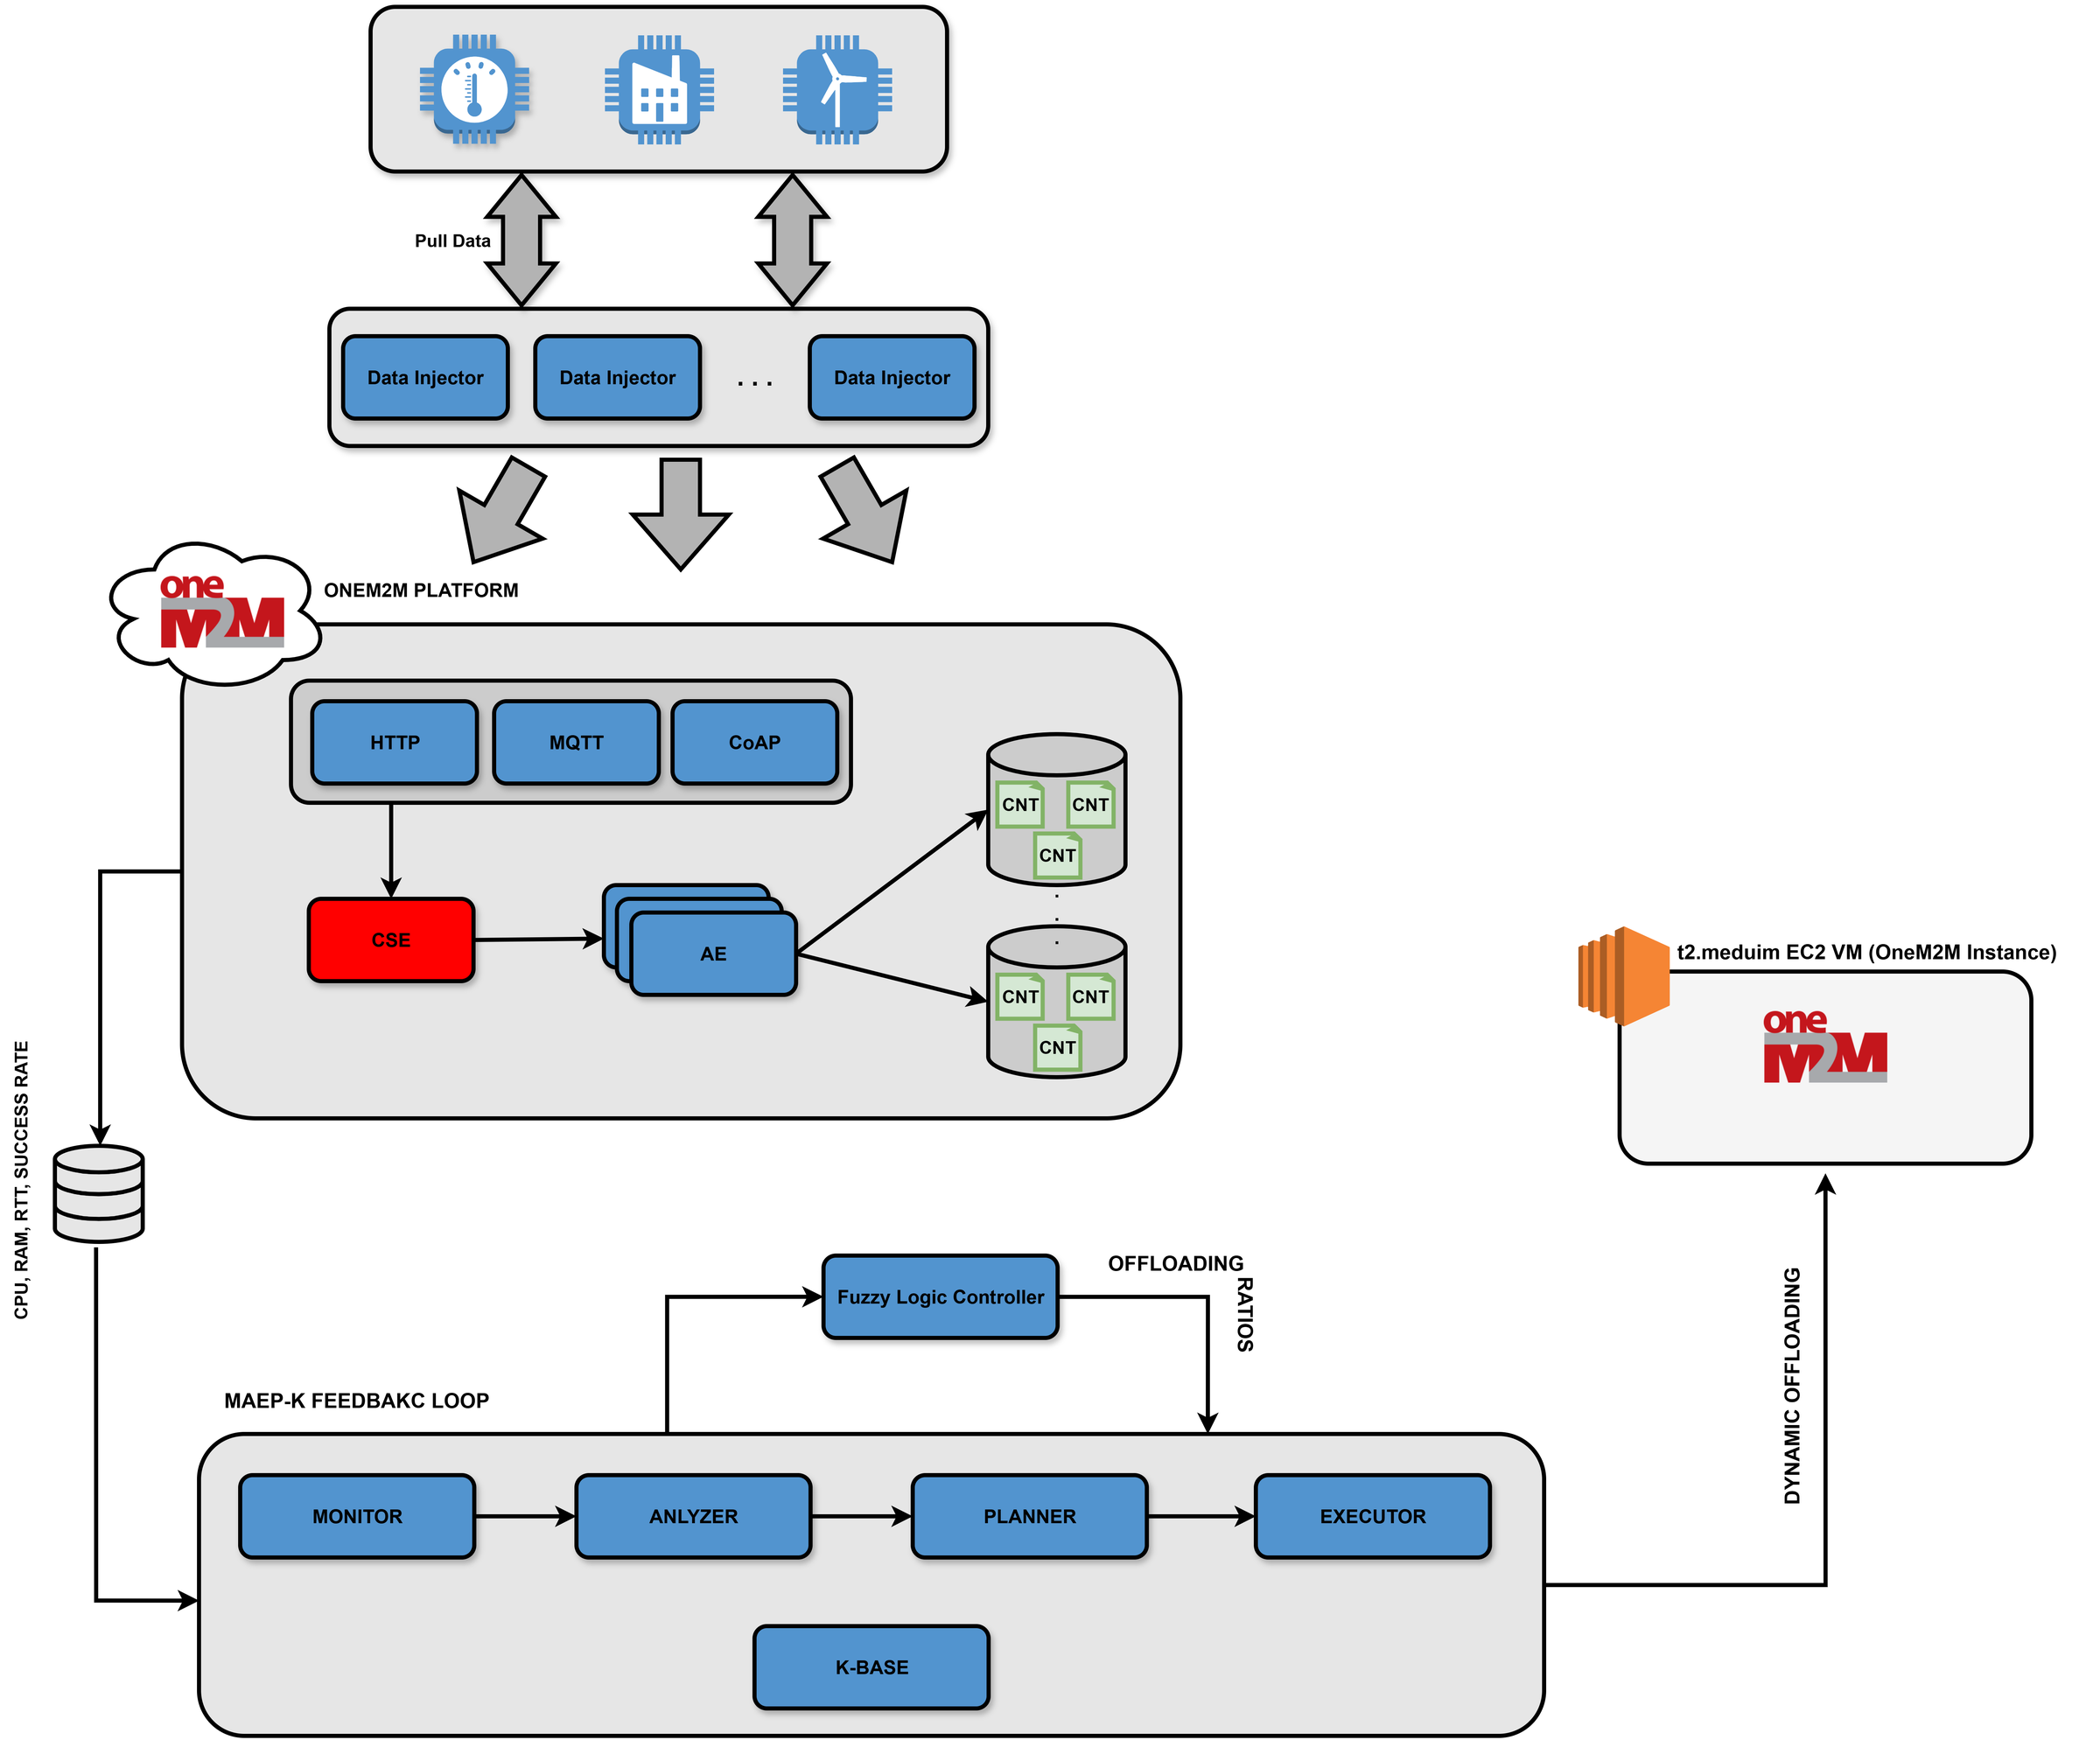
\includegraphics[width=\linewidth]{figs/paper/fig1_architecture.png}
    \end{column}
    \begin{column}{0.42\textwidth}
      \small
      \begin{enumerate}
        \item \textbf{Devices} (sensors, factory, wind turbine) feed \textbf{data injectors}.
        \item The \textbf{edge oneM2M platform}: protocol bindings $\rightarrow$ CSE $\rightarrow$ AEs $\rightarrow$ containers.
        \item A \textbf{database} stores CPU / RAM / RTT / success rate.
        \item The \textbf{MAPE-K loop} with the \textbf{Fuzzy Logic Controller} watches it all.
        \item Offloaded traffic goes to a second \textbf{oneM2M instance on AWS}.
      \end{enumerate}
    \end{column}
  \end{columns}
\end{frame}

% -----------------------------------------------------------------------------
\begin{frame}{Same picture, three layers}
  \slideid{layers}
  \centering
  \begin{tikzpicture}[node distance=0.5cm]
    % devices
    \node[box=cNormal,minimum width=12.5cm,minimum height=0.9cm] (dev) {\textbf{Device layer}\quad sensors, meters, machines $\rightarrow$ small oneM2M CREATE requests};
    % edge
    \node[draw=mcmPrimary,fill=mcmPrimary!6,rounded corners=4pt,minimum width=8.3cm,minimum height=3.2cm,below=0.9cm of dev.south west,anchor=north west] (edge) {};
    \node[anchor=north west,font=\small\bfseries,text=mcmPrimary] at (edge.north west) {\;Edge layer: local oneM2M (Mobius)};
    \node[box,minimum width=2.2cm,minimum height=1.0cm] (cse) at ([xshift=1.55cm,yshift=0.35cm]edge.west) {CSE + AEs\\\scriptsize serves requests};
    \node[draw=cBase,fill=cBase!10,rounded corners=3pt,minimum width=4.9cm,minimum height=1.9cm,align=center] (aqm) at ([xshift=-2.75cm,yshift=-0.2cm]edge.east) {};
    \node[font=\scriptsize\bfseries,text=cBase!80!black,anchor=north] at (aqm.north) {Autonomic QoS Manager};
    \foreach \l/\x in {M/-1.8,A/-0.9,P/0,E/0.9}{
      \node[circle,fill=cBase,text=white,font=\scriptsize\bfseries,inner sep=1.5pt,minimum size=0.55cm] (m\l) at ([xshift=\x cm,yshift=-0.05cm]aqm.center) {\l};}
    \node[circle,fill=mcmBlack!70,text=white,font=\scriptsize\bfseries,minimum size=0.55cm,inner sep=1pt] (mK) at ([xshift=1.8cm,yshift=-0.05cm]aqm.center) {K};
    \draw[-Stealth,thick,cBase] (mM)--(mA); \draw[-Stealth,thick,cBase] (mA)--(mP); \draw[-Stealth,thick,cBase] (mP)--(mE);
    \node[font=\tiny\bfseries,text=cBase!80!black,below=0.05cm of mP] {FLC};
    % cloud
    \node[box=spJohn,minimum width=3.6cm,minimum height=3.2cm,anchor=north west] (cloud) at ([xshift=0.6cm]edge.north east) {\textbf{Cloud layer}\\[3pt]\scriptsize oneM2M on AWS\\\scriptsize t2.medium\\[3pt]\scriptsize big, elastic,\\\scriptsize pay per hour};
    \draw[arr] ([xshift=-2cm]dev.south) -- ([xshift=-2cm]dev.south |- edge.north);
    \draw[arr,line width=1.6pt,cBase] (edge.east |- cse) -- node[above,font=\scriptsize\bfseries,text=cBase]{$\alpha$} (cloud.west |- cse);
    \draw[arr,line width=1.6pt] (edge.east |- cse) ++(-8.3cm,0) ;
    \draw[-Stealth,thick,mcmBlack!45,dashed] (cse.east) -- node[above,font=\tiny]{metrics} (aqm.west);
  \end{tikzpicture}

  \vspace{4pt}
  {\small $1-\alpha$ of the traffic stays at the edge, $\alpha$ goes to the cloud. Only $\alpha$ is decided.}
\end{frame}

% -----------------------------------------------------------------------------
\begin{frame}{Edge layer vs.\ cloud layer}
  \slideid{edgecloud}
  \centering
  \renewcommand{\arraystretch}{1.35}
  \begin{tabular}{>{\bfseries}l p{5.2cm} p{5.2cm}}
    \toprule
     & {\color{mcmPrimary}\textbf{Edge}} & {\color{spJohn}\textbf{Cloud}} \\
    \midrule
    Where & Gateways, small servers next to devices & Data centres, far away \\
    Strength & Low delay, no cloud bill & Lots of CPU, storage, networking \\
    Weakness & Small: saturates under bursts & Extra latency and a per-hour cost \\
    Best for & Time-sensitive, light work & Heavy work, overflow during peaks \\
    In the paper & Ubuntu 22.04, 4 vCPU, 4\,GiB + Mobius & AWS EC2 t2.medium + Mobius \\
    \bottomrule
  \end{tabular}

  \vspace{0.5cm}
  {\small\color{mcmPrimary}\textbf{Goal:} use the edge as much as possible, the cloud only as much as needed.}
\end{frame}

% -----------------------------------------------------------------------------
\begin{frame}{How a request and a decision flow (paper, Fig.\,2)}
  \slideid{workflow}
  \centering
  \begin{tikzpicture}[node distance=0.32cm,
      st/.style={box=mcmPrimary,minimum height=0.95cm,text width=1.85cm,font=\scriptsize},
      lp/.style={box=cBase,minimum height=0.8cm,text width=1.55cm,font=\scriptsize}]
    \node[st] (a) {IoT data\\sources};
    \node[st,right=of a] (b) {Data\\injectors};
    \node[st,right=of b] (c) {oneM2M\\platform (CSE)};
    \node[st,right=of c] (d) {AEs and\\containers};
    \node[st,right=of d,text width=2.3cm] (e) {Database\\CPU, RAM, RTT,\\success rate};
    \foreach \u/\v in {a/b,b/c,c/d,d/e} \draw[arr] (\u)--(\v);
    \node[lp,below=1.3cm of e] (m) {Monitor};
    \node[lp,left=0.45cm of m] (an) {Analyzer};
    \node[lp,left=0.45cm of an,draw=cBase,fill=cBase!30] (p) {Planner\\+ FLC};
    \node[lp,left=0.45cm of p] (ex) {Executor};
    \node[st,left=0.45cm of ex,draw=spJohn,fill=spJohn!10,text width=2.0cm] (dec) {Cloud\\offloading\\decision};
    \node[lp,below=0.45cm of an,fill=mcmBlack!8,draw=mcmBlack!50] (k) {Knowledge\\base};
    \draw[arr] (e)--(m); \draw[arr] (m)--(an); \draw[arr] (an)--(p); \draw[arr] (p)--(ex); \draw[arr] (ex)--(dec);
    \draw[arr,dashed] (dec.north) -- ++(0,0.55) -| node[pos=0.25,above,font=\tiny]{re-route $\alpha$ of the traffic} (c.south);
    \draw[mcmBlack!40,thick,dashed] (k.west) -| (p.south); \draw[mcmBlack!40,thick,dashed] (k.east) -| (m.south);
  \end{tikzpicture}

  \vspace{4pt}
  {\small Top row: the data path. Bottom row: the control loop that watches it and changes the routing.}
\end{frame}

% -----------------------------------------------------------------------------
\begin{frame}{The Autonomic QoS Manager: a MAPE-K loop}
  \slideid{mapek}
  \begin{columns}[c]
    \begin{column}{0.47\textwidth}
      \centering
      \begin{tikzpicture}
        \node[circle,fill=mcmBlack!75,text=white,minimum size=1.7cm,font=\small\bfseries,align=center] (K) at (0,0) {Know-\\ledge};
        \foreach \a/\n/\l in {135/M/Monitor,45/A/Analyze,-45/P/Plan,-135/E/Execute}{
          \node[circle,fill=mcmPrimary,text=white,minimum size=1.35cm,font=\scriptsize\bfseries] (\n) at (\a:2.25) {\l};}
        \draw[-{Stealth[length=7pt]},line width=1.6pt,mcmPrimary!60] (M) to[bend left=28] (A);
        \draw[-{Stealth[length=7pt]},line width=1.6pt,mcmPrimary!60] (A) to[bend left=28] (P);
        \draw[-{Stealth[length=7pt]},line width=1.6pt,mcmPrimary!60] (P) to[bend left=28] (E);
        \draw[-{Stealth[length=7pt]},line width=1.6pt,mcmPrimary!60] (E) to[bend left=28] (M);
        \foreach \n in {M,A,P,E} \draw[mcmBlack!35,thick,dashed] (K)--(\n);
        \node[tag=cBase] at ($(P)+(0.0,-0.95)$) {fuzzy controller};
        \node[font=\scriptsize,text=mcmBlack!60] at (0,3.3) {one turn every 5\,s};
      \end{tikzpicture}
    \end{column}
    \begin{column}{0.51\textwidth}
      \footnotesize
      \begin{description}[Execute]
        \item[\color{mcmPrimary}Monitor] Collect CPU, RAM, RTT, queue length, bandwidth from the platform and edge nodes.
        \item[\color{mcmPrimary}Analyze] Clean and normalise the numbers; spot coming overload.
        \item[\color{mcmPrimary}Plan] The \textbf{Fuzzy Logic Controller} turns the state into an offloading share $\alpha$.
        \item[\color{mcmPrimary}Execute] Re-route that share of traffic to the cloud CSE.
        \item[\color{mcmBlack!75}Knowledge] Shared store: policies, rules, history of past decisions.
      \end{description}
    \end{column}
  \end{columns}
\end{frame}

% -----------------------------------------------------------------------------
\begin{frame}{Hand-off: open the ``Plan'' box}
  \slideid{handoff2}
  \centering
  \begin{tikzpicture}
    \node[draw=mcmPrimary,line width=1pt,rounded corners=4pt,minimum width=3.0cm,minimum height=1.6cm,align=center] (in) {\textbf{measured state}\\\scriptsize CPU, RTT, traffic};
    \node[draw=spAshutosh,fill=spAshutosh!12,line width=1.5pt,rounded corners=4pt,minimum width=4.0cm,minimum height=2.0cm,right=1.2cm of in,align=center,font=\Large\bfseries,text=spAshutosh] (box) {?};
    \node[draw=mcmPrimary,line width=1pt,rounded corners=4pt,minimum width=3.0cm,minimum height=1.6cm,right=1.2cm of box,align=center] (out) {\textbf{one number}\\\scriptsize $\alpha \in [0,1]$};
    \draw[arr] (in)--(box); \draw[arr] (box)--(out);
    \node[below=0.15cm of box,font=\small\bfseries,text=spAshutosh] {Fuzzy Logic Controller};
  \end{tikzpicture}

  \vspace{0.8cm}
  {\large Everything so far is plumbing. The interesting part is \textbf{how $\alpha$ is chosen}.}\\[6pt]
  {\small\muted{Over to Ashutosh.}}
\end{frame}

% =============================================================================
% 03  ASHUTOSH: fuzzy logic controller and methodology
% =============================================================================
\usespeaker{spAshutosh}{03 Ashutosh}
\speakerpart{spAshutosh}{03}{Ashutosh}{The fuzzy logic controller and methodology}{%
  why fuzzy \textbullet{} inputs and output $\alpha(t)$ \textbullet{} membership functions \textbullet{}
  the 27-rule base (Table I) \textbullet{} inference and defuzzification \textbullet{} a worked example \textbullet{}
  monotonicity principles \textbullet{} testbed and controller configuration}

% -----------------------------------------------------------------------------
\begin{frame}{Why fuzzy? Is 69\,\% CPU ``high''?}
  \slideid{whyfuzzy}
  \begin{columns}[c]
    \begin{column}{0.48\textwidth}
      \centering
      {\small\bfseries Crisp threshold}\\[2pt]
      \begin{tikzpicture}
        \begin{axis}[width=6.3cm,height=3.7cm,axis lines=left,xmin=0,xmax=100,ymin=0,ymax=1.15,
          xlabel={CPU (\%)},ylabel={``high''},ytick={0,1},xtick={0,50,70,100},
          every axis label/.style={font=\scriptsize},tick label style={font=\scriptsize}]
          \addplot[cBase,line width=1.8pt,const plot] coordinates {(0,0) (70,0) (70,1) (100,1)};
          \addplot[only marks,mark=*,mark size=2.5pt,mcmBlack] coordinates {(69,0) (71,1)};
        \end{axis}
      \end{tikzpicture}\\
      {\scriptsize 69\,\% = ``not high'', 71\,\% = ``high''.\\Two nearly equal states, opposite actions.}
    \end{column}
    \begin{column}{0.48\textwidth}
      \centering
      {\small\bfseries Fuzzy set}\\[2pt]
      \begin{tikzpicture}
        \begin{axis}[width=6.3cm,height=3.7cm,axis lines=left,xmin=0,xmax=100,ymin=0,ymax=1.15,
          xlabel={CPU (\%)},ylabel={``high''},ytick={0,0.5,1},xtick={0,60,80,100},
          every axis label/.style={font=\scriptsize},tick label style={font=\scriptsize}]
          \addplot[cFLC,line width=1.8pt] coordinates {(0,0) (60,0) (80,1) (100,1)};
          \addplot[only marks,mark=*,mark size=2.5pt,mcmBlack] coordinates {(69,0.45) (71,0.55)};
        \end{axis}
      \end{tikzpicture}\\
      {\scriptsize 69\,\% is 0.45 high, 71\,\% is 0.55 high.\\Small change in, small change out.}
    \end{column}
  \end{columns}
  \vspace{6pt}
  \centering{\small Fuzzy logic turns expert sentences (``if CPU is high and RTT is high, offload a lot'') into a smooth controller, \textbf{no exact system model needed}.}
\end{frame}

% -----------------------------------------------------------------------------
\begin{frame}{The controller in one line}
  \slideid{flcpipe}
  \centering
  \begin{tikzpicture}[node distance=0.55cm,
      stage/.style={box=mcmPrimary,minimum height=1.5cm,text width=2.15cm,font=\scriptsize}]
    \node[align=left,font=\scriptsize] (in) {$x_1$: CPU (\%)\\[3pt]$x_2$: RTT (ms)\\[3pt]$x_3$: traffic (msg/s)};
    \node[stage,right=of in] (f) {\textbf{1. Fuzzify}\\numbers $\rightarrow$\\degrees of L, M, H};
    \node[stage,right=of f] (r) {\textbf{2. Rules}\\27 IF--THEN\\rules fire};
    \node[stage,right=of r] (i) {\textbf{3. Infer}\\min for AND,\\max to combine};
    \node[stage,right=of i] (d) {\textbf{4. Defuzzify}\\centroid $\rightarrow$\\one number};
    \node[right=of d,font=\Large\bfseries,text=mcmPrimary] (o) {$\alpha(t)$};
    \foreach \u/\v in {in/f,f/r,r/i,i/d,d/o} \draw[arr] (\u)--(\v);
  \end{tikzpicture}

  \vspace{0.6cm}
  \begin{columns}[T]
    \begin{column}{0.45\textwidth}
      \begin{block}{Output}
        \small $\alpha(t) \in [0,1]$: share of incoming traffic sent from the local oneM2M platform to the cloud.\\
        $\alpha=0$: all local. \quad $\alpha=1$: all to cloud.
      \end{block}
    \end{column}
    \begin{column}{0.45\textwidth}
      \begin{block}{Ranges used}
        \small CPU $\in [0, 100]$\,\%\\
        RTT $\in [0, T_{\max}]$, \; $T_{\max}=10$\,s\\
        Traffic $\in [0, R_{\max}]$, \; $R_{\max}=1000$\,msg/s
      \end{block}
    \end{column}
  \end{columns}
\end{frame}

% -----------------------------------------------------------------------------
\begin{frame}{Step 1: membership functions}
  \slideid{mf}
  \centering
  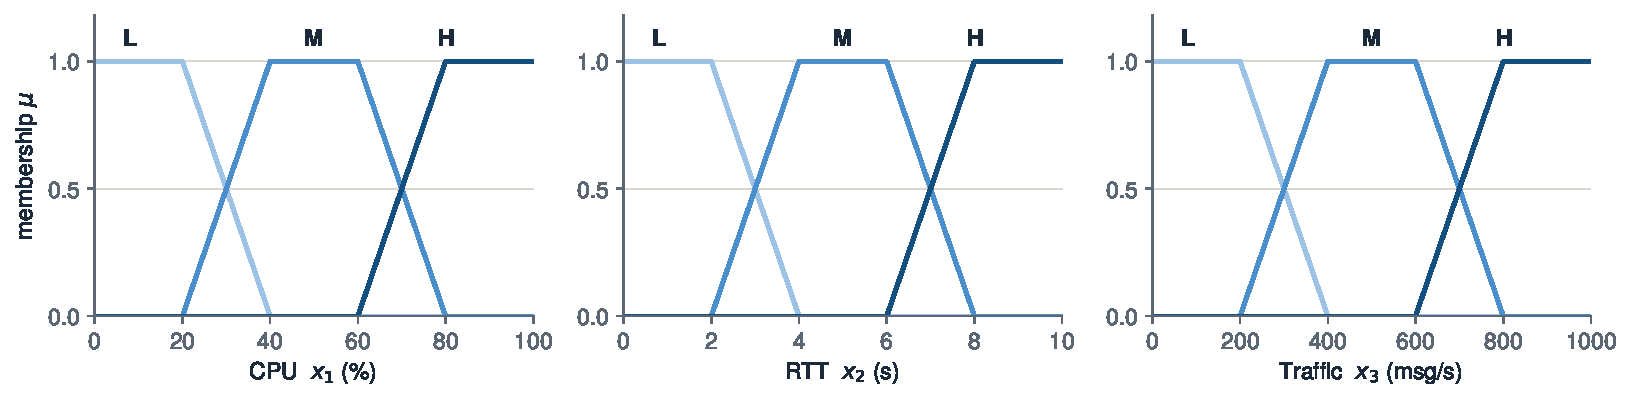
\includegraphics[width=\textwidth]{figs/gen/mf_inputs.pdf}\\[2pt]
  \begin{columns}[c]
    \begin{column}{0.55\textwidth}
      \footnotesize
      \[ \mathrm{trap}(x;a,b,c,d)=\max\!\Big(\min\!\Big(\tfrac{x-a}{b-a},\,1,\,\tfrac{d-x}{d-c}\Big),0\Big) \]
      Breakpoints at 0, 20, 40, 60, 80, 100\,\% of each range, e.g.\\
      $\mu_{\text{CPU-M}}(x_1)=\mathrm{trap}(x_1;20,40,60,80)$
    \end{column}
    \begin{column}{0.4\textwidth}
      \footnotesize Uniform partition, then light hand-tuning of $T_{\max}$, $R_{\max}$ and the high-end thresholds on held-out calibration traces.\\
      \muted{Neighbouring sets overlap, so a value can be partly M and partly H.}
    \end{column}
  \end{columns}
\end{frame}

% -----------------------------------------------------------------------------
\begin{frame}{The output: five levels of offloading}
  \slideid{mfout}
  \begin{columns}[c]
    \begin{column}{0.52\textwidth}
      \centering
      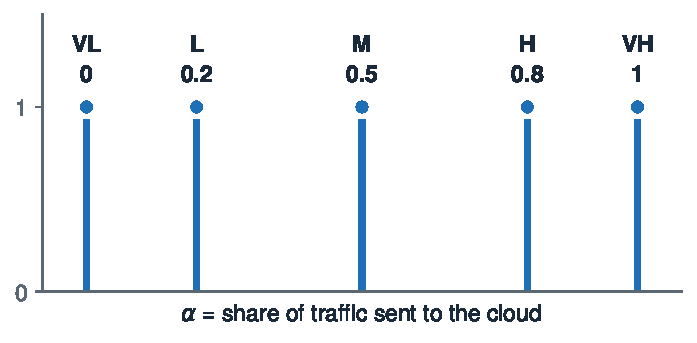
\includegraphics[width=\linewidth]{figs/gen/mf_output.pdf}
    \end{column}
    \begin{column}{0.45\textwidth}
      \small
      \begin{itemize}
        \item Five terms: Very Low, Low, Medium, High, Very High.
        \item Each is a \textbf{singleton}: a spike at one value.\\
              $\{0.0,\;0.2,\;0.5,\;0.8,\;1.0\}$
        \item Inputs are Mamdani-style fuzzy sets, outputs are Sugeno-style spikes: cheap to defuzzify.
      \end{itemize}
    \end{column}
  \end{columns}
\end{frame}

% -----------------------------------------------------------------------------
\begin{frame}{Step 2: the 27-rule base (Table I)}
  \slideid{rules}
  \begin{columns}[c]
    \begin{column}{0.66\textwidth}
      \centering
      \begin{tikzpicture}[scale=0.82,every node/.style={transform shape}]
        % CPU L
        \foreach \r/\y in {L/0,M/1,H/2} \node[font=\scriptsize,text=mcmBlack!60] at (-0.3,\y+0.5) {\r};
        \node[font=\scriptsize,text=mcmBlack!60,rotate=90] at (-0.75,1.5) {RTT $\rightarrow$};
        \ruleslice{0}{L}
        \rulecell{0}{0}{VL}\rulecell{1}{0}{VL}\rulecell{2}{0}{L}
        \rulecell{0}{1}{VL}\rulecell{1}{1}{L}\rulecell{2}{1}{M}
        \rulecell{0}{2}{L}\rulecell{1}{2}{M}\rulecell{2}{2}{H}
        \ruleslice{3.8}{M}
        \rulecell{3.8}{0}{L}\rulecell{4.8}{0}{L}\rulecell{5.8}{0}{M}
        \rulecell{3.8}{1}{L}\rulecell{4.8}{1}{M}\rulecell{5.8}{1}{H}
        \rulecell{3.8}{2}{M}\rulecell{4.8}{2}{H}\rulecell{5.8}{2}{VH}
        \ruleslice{7.6}{H}
        \rulecell{7.6}{0}{M}\rulecell{8.6}{0}{H}\rulecell{9.6}{0}{VH}
        \rulecell{7.6}{1}{H}\rulecell{8.6}{1}{VH}\rulecell{9.6}{1}{VH}
        \rulecell{7.6}{2}{VH}\rulecell{8.6}{2}{VH}\rulecell{9.6}{2}{VH}
      \end{tikzpicture}
    \end{column}
    \begin{column}{0.32\textwidth}
      \small
      $3\times3\times3 = 27$ rules, every combination covered.\\[6pt]
      Each rule reads:\\
      {\footnotesize\itshape IF CPU is $A_k$ AND RTT is $B_k$ AND traffic is $C_k$ THEN $\alpha$ is $D_k$}\\[6pt]
      {\footnotesize Written from expert knowledge of oneM2M QoS behaviour.\\
      Darker = offload more. It only gets darker as you go \textbf{up}, \textbf{right}, or to the next \textbf{CPU} grid.}
    \end{column}
  \end{columns}
\end{frame}

% -----------------------------------------------------------------------------
\begin{frame}{Step 3 and 4: inference and defuzzification}
  \slideid{inference}
  \begin{columns}[T]
    \begin{column}{0.5\textwidth}
      \begin{block}{Firing strength of rule $k$ (Zadeh AND)}
        \[ w_k(t)=\min\big(\mu_{A_k}(x_1),\,\mu_{B_k}(x_2),\,\mu_{C_k}(x_3)\big) \]
        \small A rule is only as true as its weakest condition.
      \end{block}
      \begin{block}{Combine rules with the same output (max)}
        \small $\mu_C(\text{VH}) = \max$ of all $w_k$ whose rule says VH, and so on for each level.
      \end{block}
    \end{column}
    \begin{column}{0.46\textwidth}
      \begin{block}{Centroid defuzzification}
        \[ \alpha(t)=\frac{\sum_i x_i\,\mu_C(x_i)}{\sum_i \mu_C(x_i)} \]
        \small $x_i \in \{0, 0.2, 0.5, 0.8, 1\}$: a weighted average of the five spikes.
      \end{block}
      \vspace{4pt}
      {\footnotesize\muted{Costs $<0.5$\,ms per cycle on a t2.medium: the controller is never the bottleneck.}}
    \end{column}
  \end{columns}
\end{frame}

% -----------------------------------------------------------------------------
\begin{frame}{Worked example (1/2): fuzzify}
  \slideid{example1}
  {\small Edge server state: \textbf{CPU = 70\,\%}, \textbf{RTT = 5\,s}, \textbf{traffic = 650 msg/s}.}\\[2pt]
  \centering
  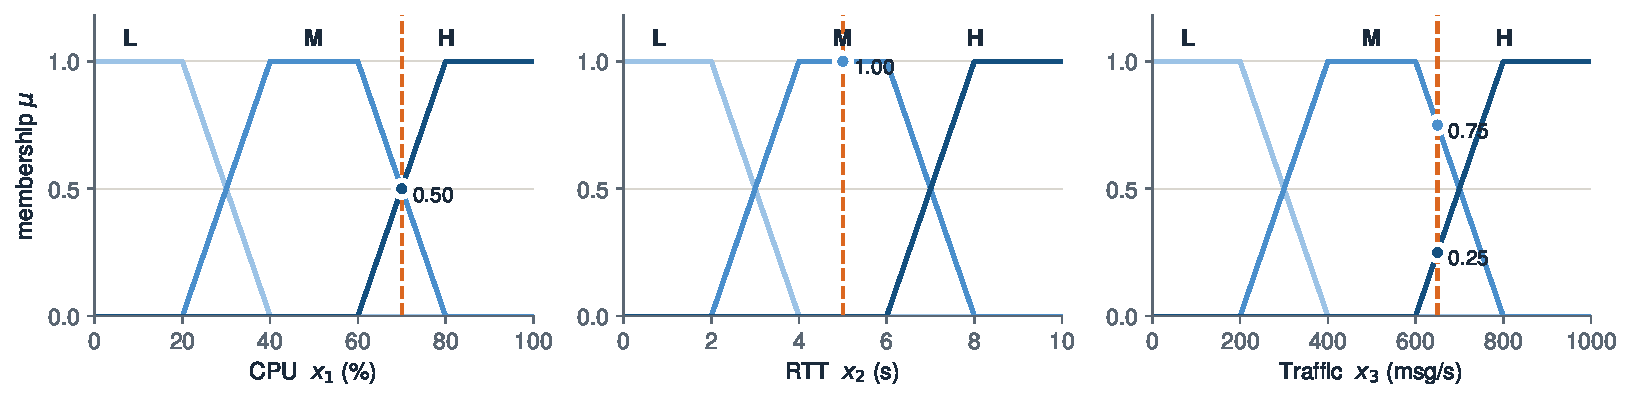
\includegraphics[width=\textwidth]{figs/gen/mf_example.pdf}\\[2pt]
  \begin{tabular}{lccc}
    & L & M & H\\\midrule
    CPU 70\,\% & 0 & \textbf{0.50} & \textbf{0.50}\\
    RTT 5\,s & 0 & \textbf{1.00} & 0\\
    Traffic 650 & 0 & \textbf{0.75} & \textbf{0.25}\\
  \end{tabular}
  \src{Computed with our re-implementation of the controller, \texttt{scripts/flc.py}.}
\end{frame}

% -----------------------------------------------------------------------------
\begin{frame}{Worked example (2/2): rules, combine, defuzzify}
  \slideid{example2}
  \begin{columns}[c]
    \begin{column}{0.5\textwidth}
      \centering\small
      \renewcommand{\arraystretch}{1.2}
      \begin{tabular}{clc}
        \toprule
        rule & IF CPU, RTT, traffic & $w_k$ \\
        \midrule
        14 & M, M, M $\rightarrow$ \textbf{M} & $\min(.5,1,.75)=0.50$\\
        15 & M, M, H $\rightarrow$ \textbf{H} & $\min(.5,1,.25)=0.25$\\
        23 & H, M, M $\rightarrow$ \textbf{VH} & $\min(.5,1,.75)=0.50$\\
        24 & H, M, H $\rightarrow$ \textbf{VH} & $\min(.5,1,.25)=0.25$\\
        \bottomrule
      \end{tabular}\\[6pt]
      {\footnotesize Other 23 rules: strength 0.}
    \end{column}
    \begin{column}{0.47\textwidth}
      \small
      Combine (max): \; M $=0.50$, \; H $=0.25$, \; VH $=0.50$\\[8pt]
      \[ \alpha=\frac{0.5\cdot0.50+0.8\cdot0.25+1.0\cdot0.50}{0.50+0.25+0.50} \]
      \[ \alpha = \frac{0.95}{1.25} = \mathbf{0.76} \]
      \begin{exampleblock}{Meaning}
        Send about \textbf{3 of every 4} requests to the cloud right now.
      \end{exampleblock}
    \end{column}
  \end{columns}
\end{frame}

% -----------------------------------------------------------------------------
\begin{frame}{The whole controller as a picture}
  \slideid{surface}
  \centering
  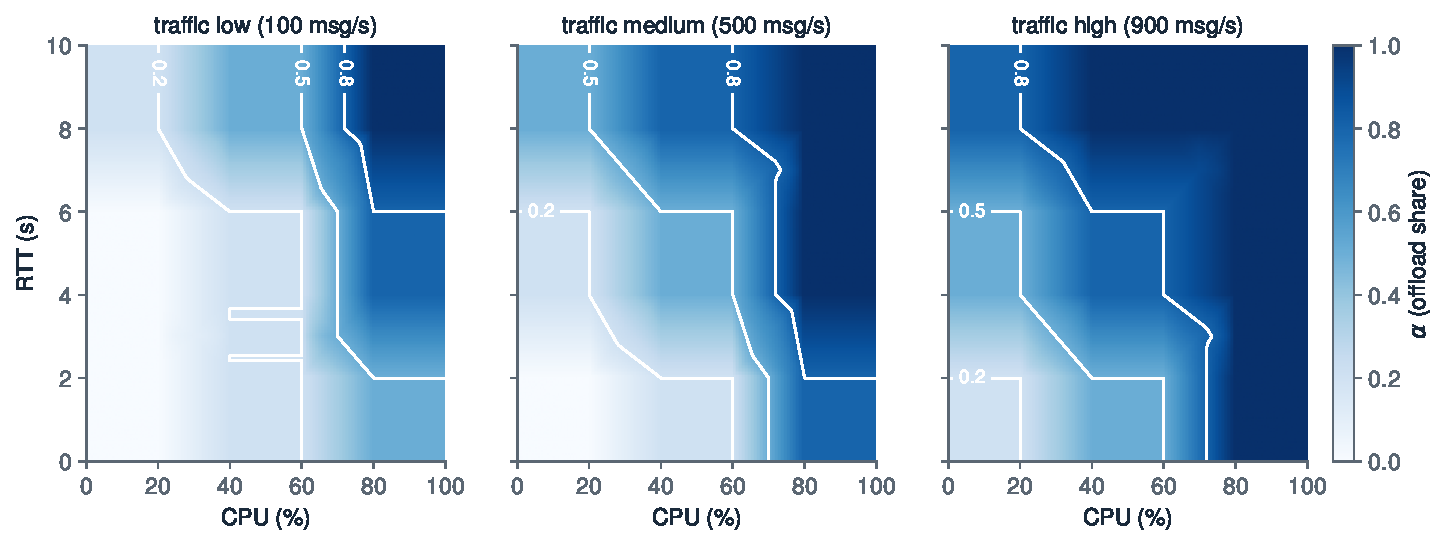
\includegraphics[width=0.98\textwidth]{figs/gen/control_surface.pdf}\\[4pt]
  {\small Darker = more offloading. The surface rises smoothly with every input: no cliffs, unlike a threshold.}
  \src{Our plot of the paper's rule base and membership functions (\texttt{scripts/make\_figs.py}).}
\end{frame}

% -----------------------------------------------------------------------------
\begin{frame}{Three design principles built into the rules}
  \slideid{monotone}
  \begin{columns}[c]
    \begin{column}{0.5\textwidth}
      \centering
      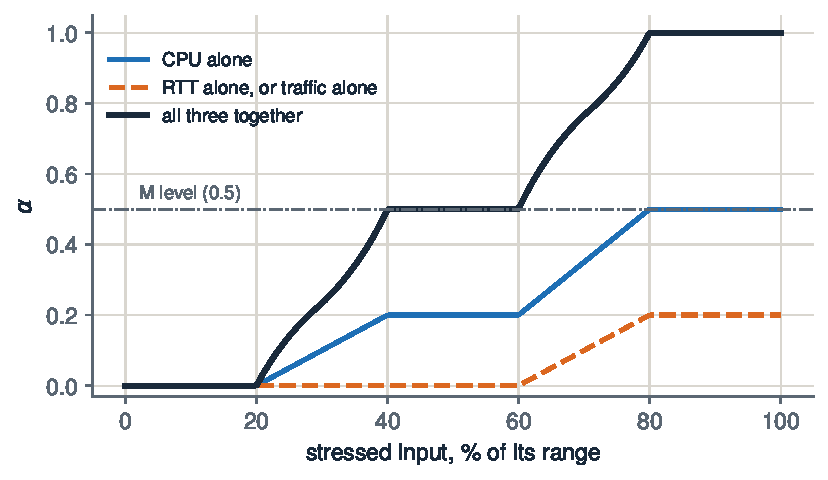
\includegraphics[width=\linewidth]{figs/gen/alpha_slices.pdf}
    \end{column}
    \begin{column}{0.48\textwidth}
      \small
      \begin{enumerate}
        \item \textbf{Monotone}: more CPU, RTT or traffic never means less offloading.
        \item \textbf{No panic on one spike}: one input saturated alone stays at or below M (0.5).\\
              {\footnotesize\muted{Robust to a single noisy sensor.}}
        \item \textbf{All three high $\Rightarrow$ $\alpha=1$}: protect the edge node.
      \end{enumerate}
      \vspace{4pt}
      {\footnotesize\muted{Curves: one input swept from 0 to 100\,\% of its range, the others held low.}}
    \end{column}
  \end{columns}
\end{frame}

% -----------------------------------------------------------------------------
\begin{frame}{Testbed and controller configuration}
  \slideid{config}
  \begin{columns}[T]
    \begin{column}{0.48\textwidth}
      \begin{block}{Testbed}
        \footnotesize
        \begin{itemize}
          \item \textbf{Edge}: Ubuntu 22.04, 4 vCPU, 4\,GiB; Mobius CSE + QoS Manager + FLC + Knowledge base.
          \item \textbf{Cloud}: Mobius CSE on AWS EC2 t2.medium.
          \item Interfaces: oneM2M Mca / Mcc over HTTP and MQTT.
          \item Monitor: CPU, RAM every 1\,s from Linux \texttt{/proc}; RTT from timestamps added by the proxy.
          \item Load: JMeter (HTTP) + Eclipse Paho (MQTT) virtual devices.
        \end{itemize}
      \end{block}
    \end{column}
    \begin{column}{0.48\textwidth}
      \begin{block}{Controller settings}
        \footnotesize
        \renewcommand{\arraystretch}{1.15}
        \begin{tabular}{@{}ll@{}}
          MAPE-K period & 5\,s ($<3$\,\% of a core)\\
          Inference & Mamdani min--max\\
          Defuzzification & centroid\\
          Input smoothing & EMA, 3 samples, $\beta=0.6$\\
          Hysteresis & act only if $|\Delta\alpha|\ge0.05$\\
          $T_{\max}$, $R_{\max}$ & 10\,s, 1000 msg/s\\
        \end{tabular}\\[4pt]
        Only the period, the smoothing and the hysteresis were tuned; the rules and breakpoints stayed fixed.
      \end{block}
    \end{column}
  \end{columns}
\end{frame}

% =============================================================================
% 04  JOHN: experimental setup and results  (kept deliberately simple)
% =============================================================================
\usespeaker{spJohn}{04 John}
\speakerpart{spJohn}{04}{John}{Did it work?}{%
  the test in one picture \textbullet{} four load levels \textbullet{} three scenarios \textbullet{}
  what happened to speed, reliability and CPU \textbullet{} what happened to the bill}

% -----------------------------------------------------------------------------
\begin{frame}{The test in one picture}
  \slideid{testpic}
  \centering
  \begin{tikzpicture}[node distance=2.3cm]
    \node[box=cNormal,minimum width=3.2cm,minimum height=2.2cm,font=\normalsize] (d) {\textbf{Fake devices}\\[2pt]\small 50 to 1000\\\small of them};
    \node[box=mcmPrimary,minimum width=3.4cm,minimum height=2.2cm,right=of d,font=\normalsize] (e) {\textbf{Edge server}\\[2pt]\small with the\\\small fuzzy brain};
    \node[box=cBase,minimum width=3.2cm,minimum height=2.2cm,right=of e,font=\normalsize] (c) {\textbf{Cloud}\\[2pt]\small Amazon\\\small (AWS)};
    \draw[arr,line width=2pt] (d)--node[above,font=\small]{requests}(e);
    \draw[arr,line width=2pt,dashed] (e)--node[above,font=\small]{overflow}(c);
  \end{tikzpicture}

  \vspace{0.8cm}
  {\Large Each run: \textbf{30 minutes}, repeated \textbf{5 times}.}
\end{frame}

% -----------------------------------------------------------------------------
\begin{frame}{Four levels of load}
  \slideid{loads}
  \centering
  \begin{tikzpicture}
    \foreach \x/\h/\n/\l in {0/0.25/50/Light,3.5/1.25/250/Medium,7/3.0/600/Heavy,10.5/5.0/1000/Peak}{
      \fill[mcmPrimary!80,rounded corners=2pt] (\x,0) rectangle ++(1.8,\h*0.8);
      \node[font=\large\bfseries,text=mcmPrimary,above] at (\x+0.9,\h*0.8) {\n};
      \node[font=\normalsize\bfseries,below] at (\x+0.9,-0.05) {\l};
    }
    \draw[mcmBlack!40,line width=0.8pt] (-0.3,0)--(12.6,0);
  \end{tikzpicture}\\[6pt]
  {\large devices, each sending about \textbf{one request per second}}
\end{frame}

% -----------------------------------------------------------------------------
\begin{frame}{Three scenarios}
  \slideid{scenarios}
  \centering
  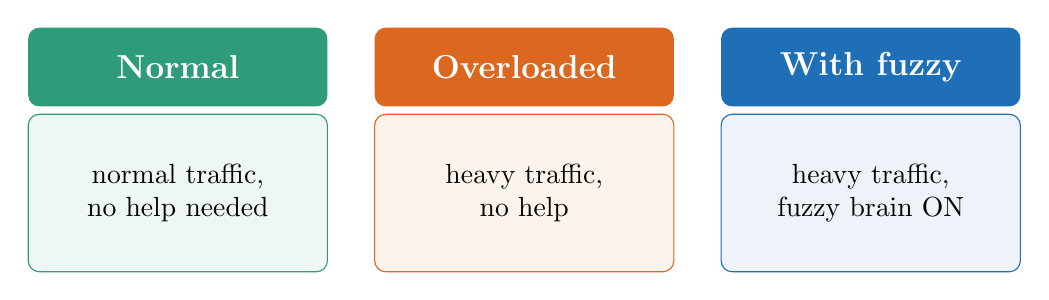
\begin{tikzpicture}
    \foreach \x/\c/\t/\s/\d in {
      0/cNormal/Normal/{\large\ding{52}}/{normal traffic,\\no help needed},
      4.4/cBase/Overloaded/{\large\ding{55}}/{heavy traffic,\\no help},
      8.8/cFLC/{With fuzzy}/{\large\ding{52}}/{heavy traffic,\\fuzzy brain ON}}{
      \node[fill=\c,text=white,rounded corners=4pt,minimum width=3.8cm,minimum height=1.0cm,font=\large\bfseries] at (\x,1.0) {\t};
      \node[draw=\c,fill=\c!8,rounded corners=4pt,minimum width=3.8cm,minimum height=2.0cm,align=center,font=\normalsize] at (\x,-0.6) {\d};
    }
  \end{tikzpicture}

  \vspace{0.7cm}
  {\large Same heavy traffic in the last two. \textbf{Only difference: the fuzzy brain.}}
\end{frame}

% -----------------------------------------------------------------------------
\begin{frame}{Speed: response time over time}
  \slideid{rttcurve}
  \begin{columns}[c]
    \begin{column}{0.62\textwidth}
      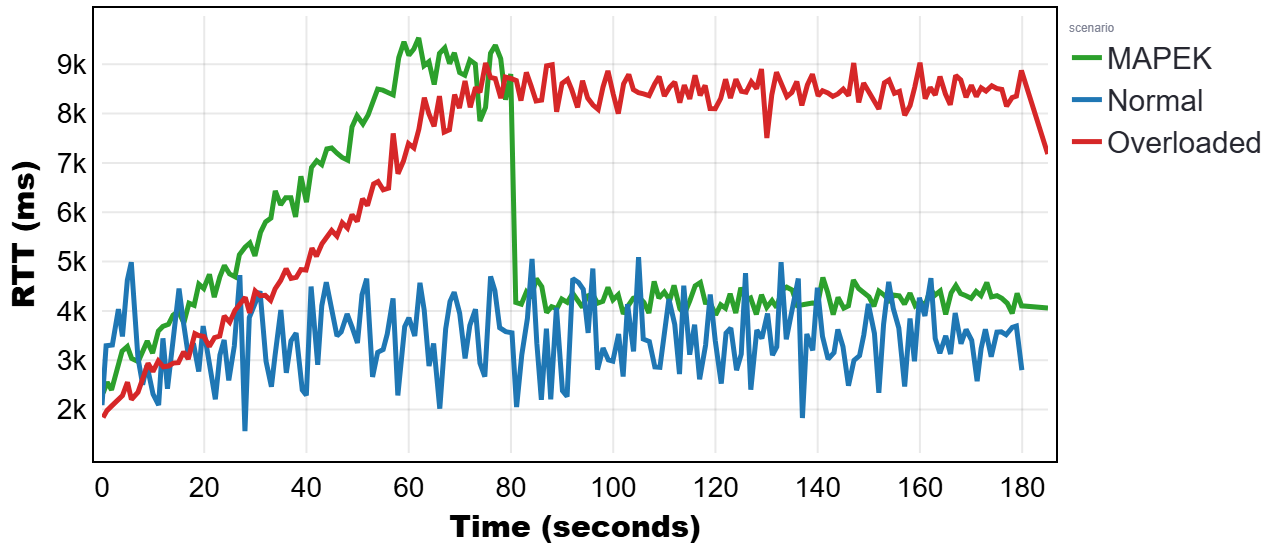
\includegraphics[width=\linewidth]{figs/paper/fig3a_rtt.png}\\
      {\tiny\muted{Paper, Fig.\,3(a)}}
    \end{column}
    \begin{column}{0.36\textwidth}
      \large
      {\color{pBlue}\textbf{Blue}}: normal.\\[6pt]
      {\color{pRed}\textbf{Red}}: overloaded, gets slow and stays slow.\\[6pt]
      {\color{pGreen}\textbf{Green}}: fuzzy brain kicks in at about 80\,s and brings it back down.
    \end{column}
  \end{columns}
\end{frame}

% -----------------------------------------------------------------------------
\begin{frame}{All three scenarios, side by side}
  \slideid{bars}
  \centering
  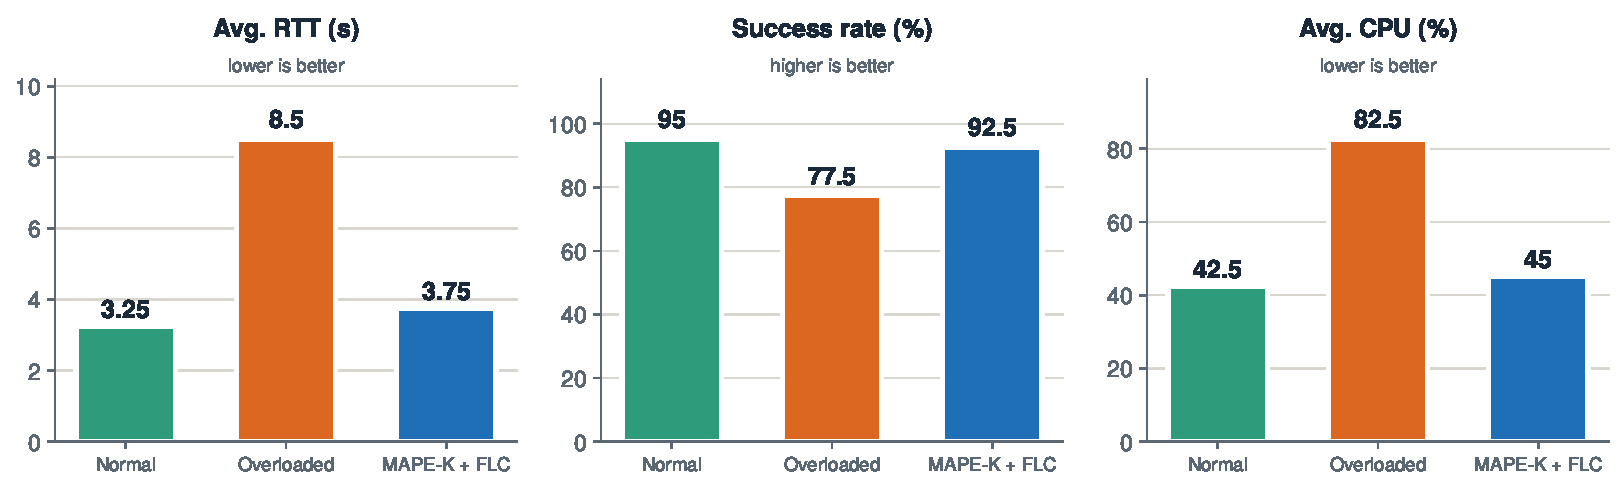
\includegraphics[width=\textwidth]{figs/gen/results_bars.pdf}\\[4pt]
  {\large Overloaded is bad on everything. \textbf{With fuzzy} is almost back to normal.}
  \src{Values from the paper's Table III; chart redrawn by us.}
\end{frame}

% -----------------------------------------------------------------------------
\begin{frame}{The bill: cloud cost per hour}
  \slideid{cost}
  \centering
  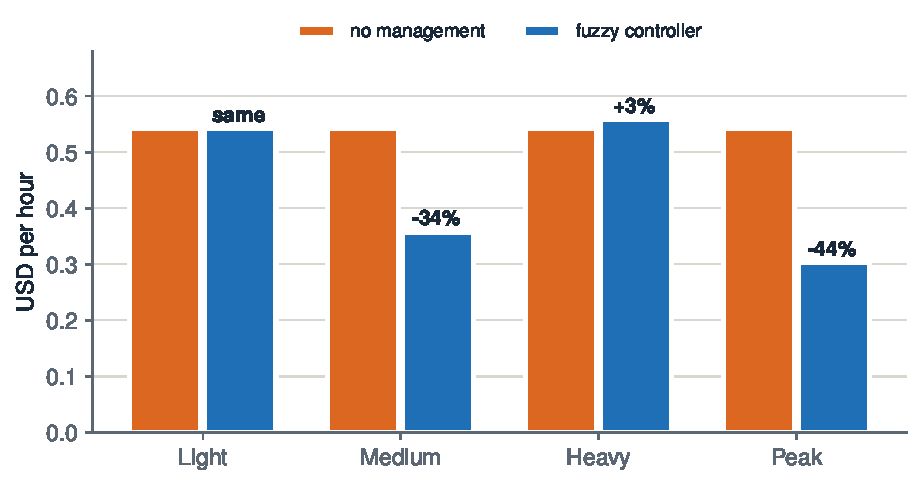
\includegraphics[width=0.75\textwidth]{figs/gen/cost_regimes.pdf}\\[4pt]
  {\large Saves money at \textbf{medium} and \textbf{peak} load.}\\
  {\small\muted{Heavy costs slightly more on purpose: it spends a little to keep service good.}}
  \src{Values from the paper's Table III; chart redrawn by us.}
\end{frame}

% -----------------------------------------------------------------------------
\begin{frame}{Three numbers to remember}
  \slideid{three}
  \centering
  \vspace{0.3cm}
  \begin{columns}[T]
    \begin{column}{0.31\textwidth}\centering
      \bignum{43.5\%}\\[4pt]{\large cheaper}
    \end{column}
    \begin{column}{0.31\textwidth}\centering
      \bignum{55.9\%}\\[4pt]{\large faster}
    \end{column}
    \begin{column}{0.31\textwidth}\centering
      \bignum{19.4\%}\\[4pt]{\large more requests succeed}
    \end{column}
  \end{columns}
  \vspace{0.9cm}

  {\large compared with doing nothing, under heavy load.}\\[10pt]
  {\small\muted{Is that good enough? Over to Ayush.}}
\end{frame}

% =============================================================================
% 05  AYUSH: comparison, critical analysis, conclusion
% =============================================================================
\usespeaker{spAyush}{05 Ayush}
\speakerpart{spAyush}{05}{Ayush}{Comparison, critical analysis and conclusion}{%
  baselines \textbullet{} static threshold vs.\ fuzzy (Fig.\,4) \textbullet{} Table IV \textbullet{}
  checking the numbers \textbullet{} our own re-simulation \textbullet{} scalability \textbullet{}
  strengths and limitations \textbullet{} summary and future work}

% -----------------------------------------------------------------------------
\begin{frame}{What it is compared against}
  \slideid{baselines}
  \begin{columns}[T]
    \begin{column}{0.32\textwidth}
      \begin{block}{1. Unmanaged}
        \small Everything processed locally. Same as the Overloaded scenario: a default Mobius install.\\[3pt]
        \muted{Worst case.}
      \end{block}
    \end{column}
    \begin{column}{0.32\textwidth}
      \begin{block}{2. Static threshold}
        \small Offload \textbf{100\,\%} when CPU $>$ 70\,\%; back to local when CPU $<$ 50\,\%.\\[3pt]
        \muted{Typical industry ``cloud bursting''.}
      \end{block}
    \end{column}
    \begin{column}{0.32\textwidth}
      \begin{block}{3. Literature}
        \small FI-RBTOM (fuzzy rules) [6], fuzzy Q-learning [7], load-balance-aware collaborative offloading [11].\\[3pt]
        \muted{Compared qualitatively only.}
      \end{block}
    \end{column}
  \end{columns}
\end{frame}

% -----------------------------------------------------------------------------
\begin{frame}{Static threshold vs.\ fuzzy: how $\alpha$ moves (paper, Fig.\,4)}
  \slideid{fig4}
  \begin{columns}[c]
    \begin{column}{0.58\textwidth}
      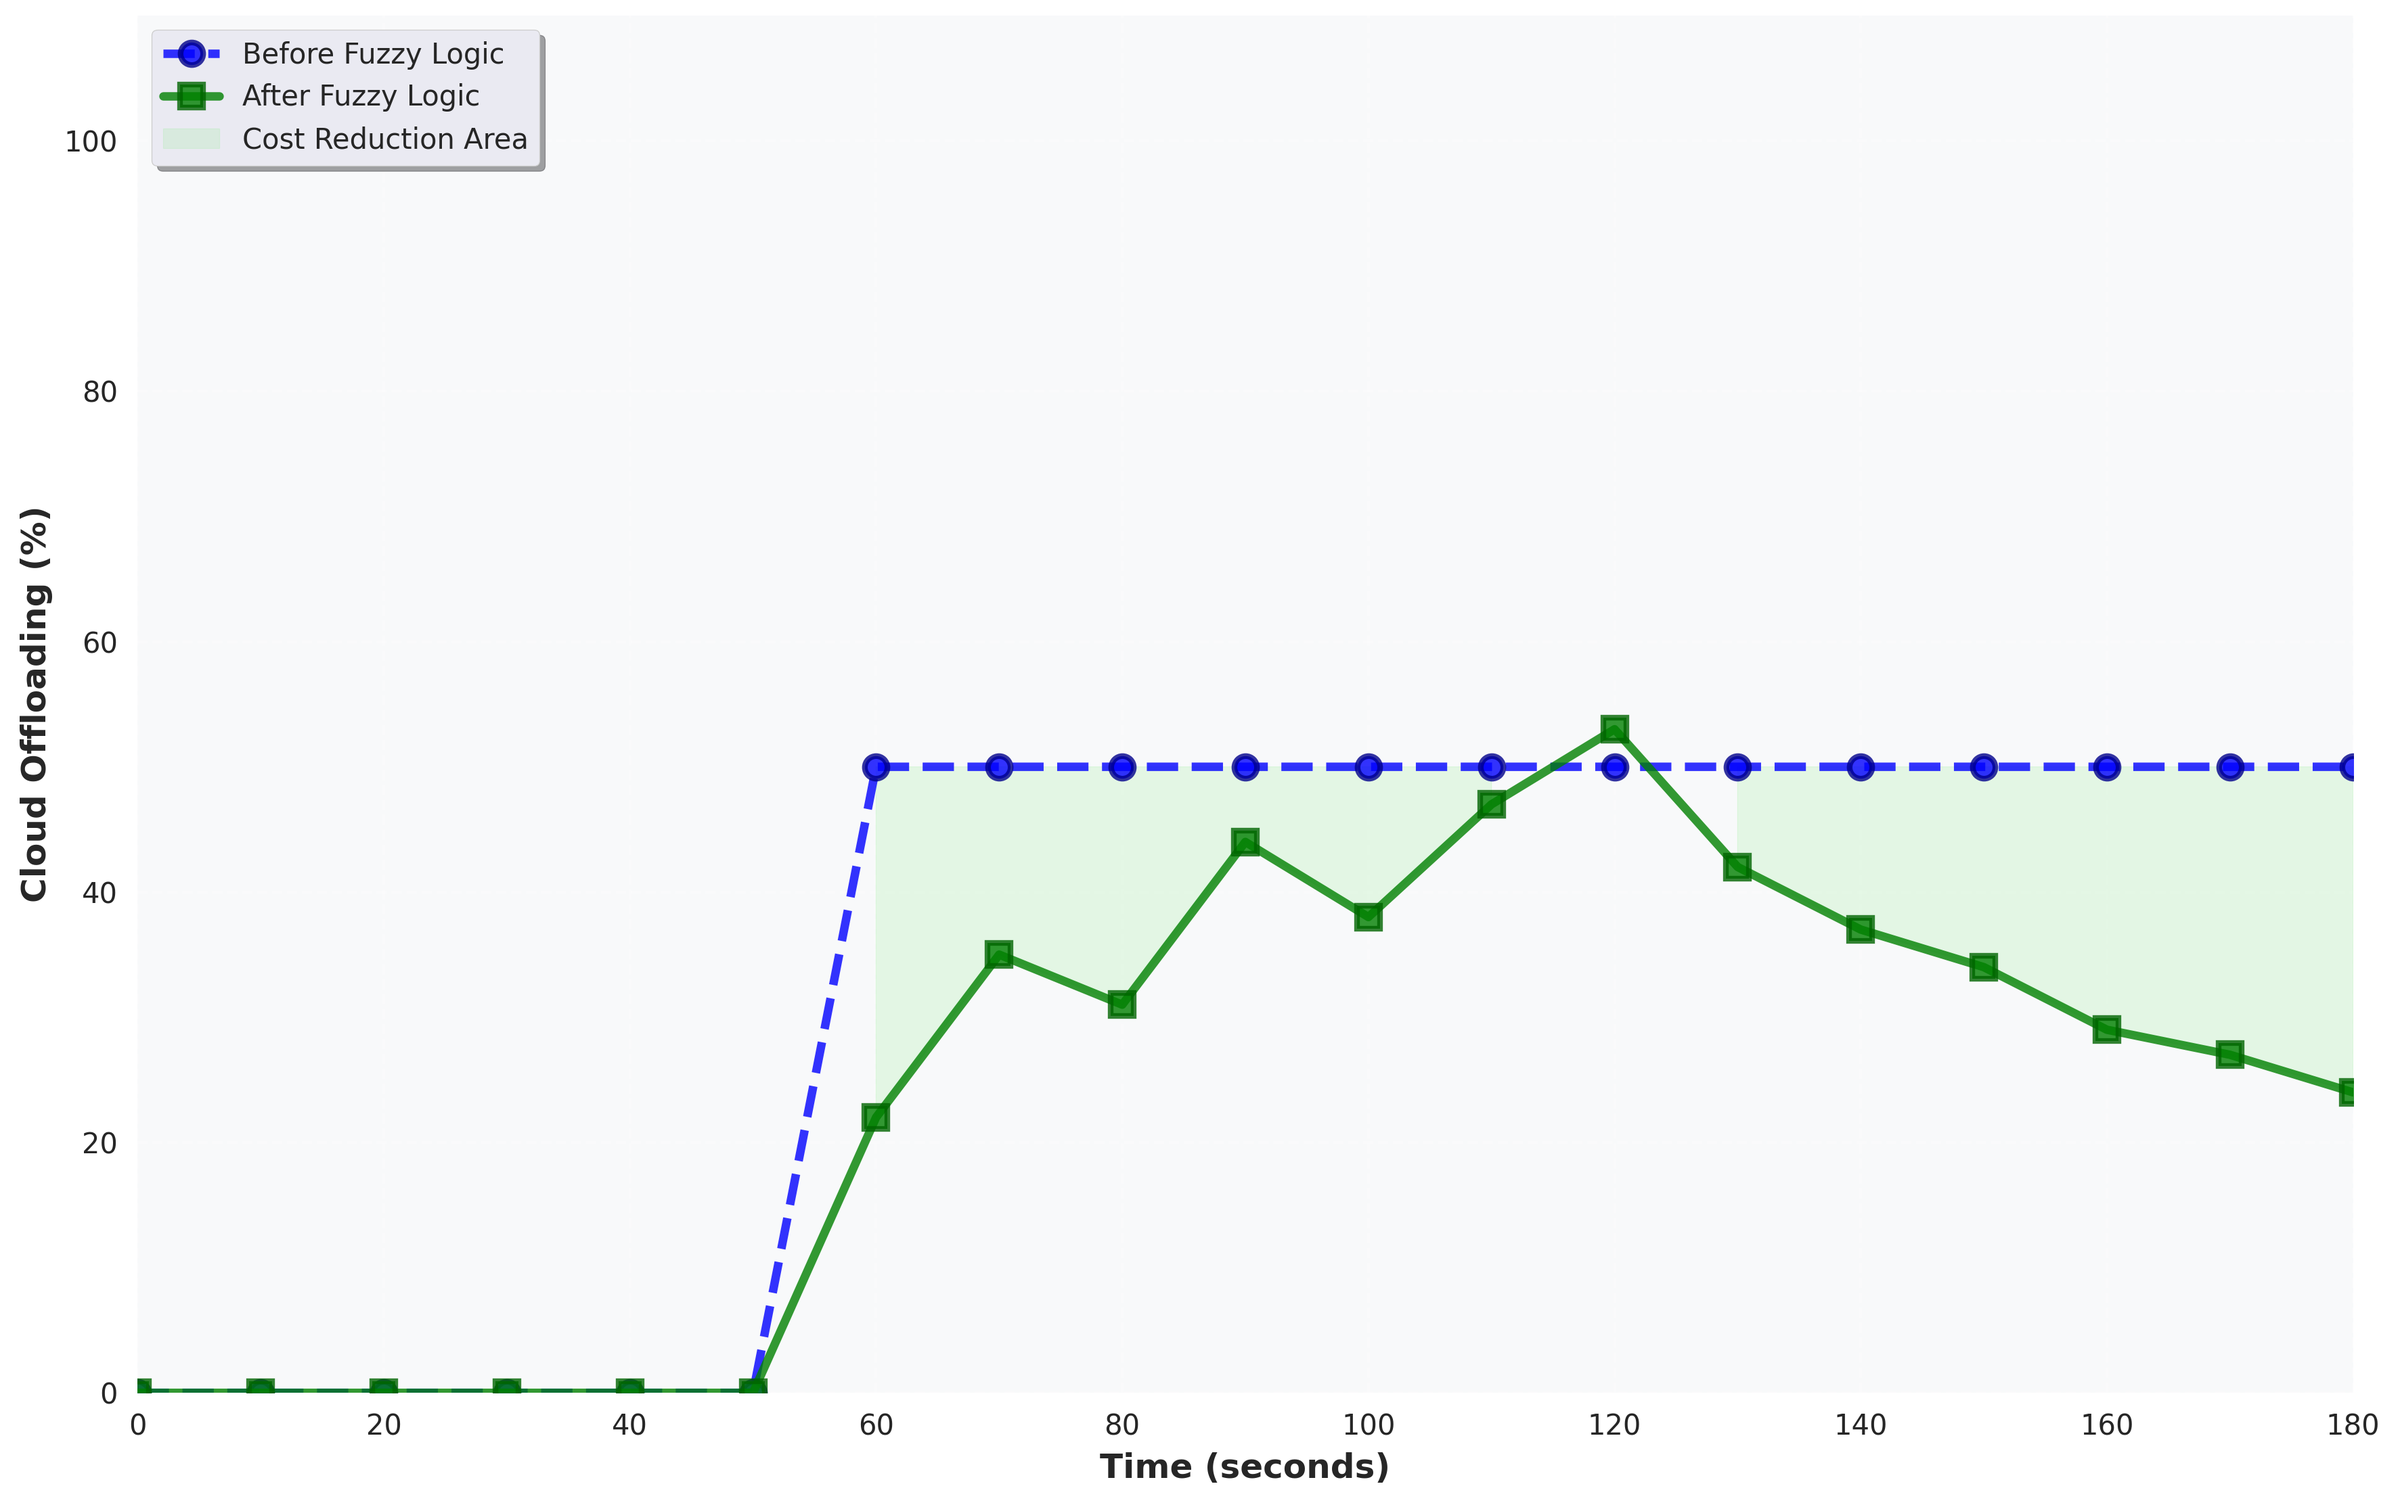
\includegraphics[width=\linewidth]{figs/paper/fig4_offload_ratio.png}
    \end{column}
    \begin{column}{0.4\textwidth}
      \small
      \begin{itemize}
        \item \textbf{Static} (dashed): 0\,\% until the CPU limit, then jumps to a fixed rate and stays there.
        \item \textbf{Fuzzy} (solid): rises with the peak, then \textbf{backs off} as load falls.
        \item Shaded area = cloud capacity the static rule pays for but does not need.
      \end{itemize}
    \end{column}
  \end{columns}
\end{frame}

% -----------------------------------------------------------------------------
\begin{frame}{Table IV, simplified}
  \slideid{table4}
  \centering\footnotesize
  \renewcommand{\arraystretch}{1.25}
  \begin{tabular}{l c c c c c c}
    \toprule
     & Unmanaged & Static & FI-RBTOM & Fuzzy QL & Collab. & \textbf{Proposed}\\
    \midrule
    RTT & 8.5\,s & better & better & better & better & \textbf{3.75\,s}\\
    Success rate & 77.5\,\% & better & better & better & better & \textbf{92.5\,\%}\\
    Cloud cost & \$2.17 & {\color{cBase}over-prov.} & n/r & lower & lower & \textbf{\$1.22}\\
    Oscillation & none & {\color{cBase}high} & moderate & low & low & \textbf{low}\\
    Inside oneM2M & native & external & external & external & external & \textbf{native}\\
    Needs training & no & no & no & {\color{cBase}yes} & no & \textbf{no}\\
    \bottomrule
  \end{tabular}\\[8pt]
  {\small Only the \textbf{Unmanaged} and \textbf{Proposed} columns are measured on this testbed.\\
  The rest is the direction of improvement reported in each cited paper.}
\end{frame}

% -----------------------------------------------------------------------------
\begin{frame}{Checking the headline numbers}
  \slideid{arith}
  \begin{columns}[T]
    \begin{column}{0.5\textwidth}
      \small
      \renewcommand{\arraystretch}{1.3}
      \begin{tabular}{@{}lccr@{}}
        \toprule
        & Overloaded & Fuzzy & change\\
        \midrule
        Total cost & \$2.1667 & \$1.2242 & \textminus43.5\,\% \cmark\\
        RTT & 8.50\,s & 3.75\,s & \textminus55.9\,\% \cmark\\
        Success & 77.5\,\% & 92.5\,\% & +19.4\,\% \cmark\\
        \bottomrule
      \end{tabular}\\[6pt]
      \footnotesize All three reproduce from Table III.\\
      But: +19.4\,\% is \emph{relative}; in absolute terms it is \textbf{+15 percentage points}.
    \end{column}
    \begin{column}{0.46\textwidth}
      \begin{block}{Where the cost comes from}
        \footnotesize
        \begin{tabular}{@{}lrr@{}}
          & before & after\\
          AWS runtime & \$0.1667 & \$0.0942\\
          Operational & \$2.0000 & \$1.1300\\
          \textbf{Total} & \textbf{\$2.1667} & \textbf{\$1.2242}\\
        \end{tabular}\\[3pt]
        t2.medium: 2 vCPU, 4\,GiB, \$0.0464/h on demand.\\
        \muted{\$0.1667 $\approx$ 3.6 instance-hours (our arithmetic). The ``operational'' cost is 92\,\% of the total but is not defined in the paper.}
      \end{block}
    \end{column}
  \end{columns}
\end{frame}

% -----------------------------------------------------------------------------
\begin{frame}{We re-implemented the controller: what a closed loop does}
  \slideid{sim}
  \begin{columns}[c]
    \begin{column}{0.6\textwidth}
      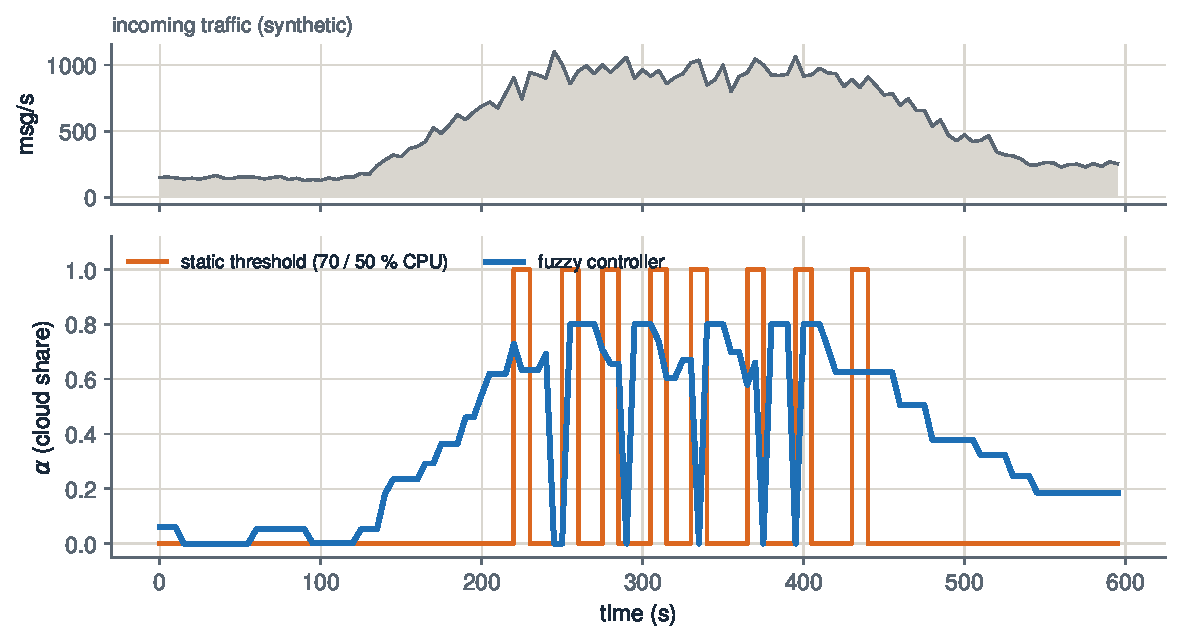
\includegraphics[width=\linewidth]{figs/gen/sim_static_vs_flc.pdf}
    \end{column}
    \begin{column}{0.38\textwidth}
      \footnotesize
      Toy edge server, same rules, EMA and hysteresis as the paper.
      \begin{itemize}
        \item \textbf{Static}: slams between 0 and 1: the bang-bang the paper warns about.
        \item \textbf{Fuzzy}: graded, follows the load up and back down.
        \item But it also \textbf{hunts}: offloading lowers CPU and RTT, which then lowers $\alpha$.
      \end{itemize}
      {\color{mcmPrimary}The paper does not analyse loop stability.}
    \end{column}
  \end{columns}
  \src{Illustration only: synthetic plant with a first-order lag, not the paper's data. Code: \texttt{scripts/make\_figs.py}.}
\end{frame}

% -----------------------------------------------------------------------------
\begin{frame}{Scaling to hundreds of edge nodes}
  \slideid{scale}
  \begin{columns}[c]
    \begin{column}{0.5\textwidth}
      \centering
      {\small\bfseries Per-node managers}\\[3pt]
      \begin{tikzpicture}[scale=0.85]
        \node[box=spJohn,minimum width=3.6cm,font=\scriptsize] (kb) at (1.5,1.7) {shared Knowledge (summaries)};
        \foreach \x in {0,1,2,3}{
          \node[circle,fill=mcmPrimary,text=white,font=\tiny\bfseries,minimum size=0.75cm] (n\x) at (\x,0) {FLC};
          \draw[mcmBlack!40,dashed] (n\x)--(kb);}
      \end{tikzpicture}\\
      {\scriptsize Fully decentralised. Traffic $O(N)$, decision latency constant.}
    \end{column}
    \begin{column}{0.48\textwidth}
      \centering
      {\small\bfseries Hierarchical FLC}\\[3pt]
      \begin{tikzpicture}[scale=0.85]
        \node[circle,fill=spAyush,text=white,font=\tiny\bfseries,minimum size=0.9cm,align=center] (top) at (1.5,1.7) {cloud\\FLC};
        \foreach \x in {0,1,2,3}{
          \node[circle,fill=mcmPrimary,text=white,font=\tiny\bfseries,minimum size=0.75cm] (m\x) at (\x,0) {FLC};
          \draw[-Stealth,mcmBlack!50] (top)--(m\x);}
      \end{tikzpicture}\\
      {\scriptsize Cloud-level FLC sets per-region offload caps; local FLCs stay independent.}
    \end{column}
  \end{columns}
  \vspace{8pt}
  \centering{\small 27 rules + centroid $<0.5$\,ms per 5\,s cycle per node. \textbf{Argued, not yet measured:} the testbed has one edge node and one cloud VM.}
\end{frame}

% -----------------------------------------------------------------------------
\begin{frame}{Critical analysis}
  \slideid{critique}
  \begin{columns}[T]
    \begin{column}{0.44\textwidth}
      \begin{exampleblock}{Strengths}
        \footnotesize
        \begin{itemize}
          \item Fully \textbf{interpretable}: 27 readable rules, no training data.
          \item Runs \textbf{inside} oneM2M (Mobius): any oneM2M app benefits unchanged.
          \item Cheap: $<0.5$\,ms per decision.
          \item Clear, sensible design principles (monotone, no single-spike panic).
          \item Improves QoS \emph{and} cost at the same time.
        \end{itemize}
      \end{exampleblock}
    \end{column}
    \begin{column}{0.53\textwidth}
      \begin{alertblock}{Limitations we found}
        \scriptsize
        \begin{itemize}
          \item \textbf{One edge node, one VM, synthetic traffic}; scalability is argued, not measured.
          \item Literature comparison is \textbf{qualitative}; the static baseline has no numbers.
          \item Means of 5 runs, \textbf{no variance}; CPU and RAM averages \textbf{identical} in every row of Table III.
          \item ``Operational'' cost (92\,\% of the bill) is never defined.
          \item Text promises bandwidth and task size as inputs; the controller uses CPU, RTT, traffic.
          \item Hand-tuned breakpoints; \textbf{loop stability} not studied (see our re-sim).
        \end{itemize}
      \end{alertblock}
    \end{column}
  \end{columns}
\end{frame}

% -----------------------------------------------------------------------------
\begin{frame}{Summary and future work}
  \slideid{summary}
  \begin{columns}[T]
    \begin{column}{0.48\textwidth}
      \begin{block}{Summary}
        \small
        \begin{itemize}
          \item A 27-rule fuzzy controller inside a MAPE-K loop decides \textbf{how much} oneM2M traffic to send to the cloud.
          \item Under overload: RTT \textminus55.9\,\%, success +19.4\,\%, cost \textminus43.5\,\%, CPU back to 40--50\,\%.
          \item A practical, low-cost option for oneM2M platforms; the evidence is still small-scale.
        \end{itemize}
      \end{block}
    \end{column}
    \begin{column}{0.48\textwidth}
      \begin{block}{Future work (from the paper)}
        \small
        \begin{enumerate}
          \item Auto-tune breakpoints and rule weights (RL or evolutionary search).
          \item Multi-objective control: QoS + energy + cost.
          \item Security-aware QoS: DDoS and anomaly signals as fuzzy inputs.
          \item Distributed / hierarchical MAPE-K on a real multi-host edge testbed.
        \end{enumerate}
      \end{block}
    \end{column}
  \end{columns}
\end{frame}

% -----------------------------------------------------------------------------
\begin{frame}[plain]
  \slideid{thanks}
  \begin{tikzpicture}[remember picture,overlay]
    \fill[mcmBg] (current page.south west) rectangle (current page.north east);
    \node[font=\mcmTitleFont\Huge,text=mcmBlack!85] at ([yshift=1.6cm]current page.center) {THANK YOU};
    \node[font=\large,text=mcmBlack!60] at ([yshift=0.6cm]current page.center) {Questions?};
    \foreach \i/\n/\c in {1/Raj/spRaj,2/Manoj/spManoj,3/Ashutosh/spAshutosh,4/John/spJohn,5/Ayush/spAyush}{
      \node[fill=\c,text=white,rounded corners=3pt,minimum width=2.3cm,minimum height=0.8cm,font=\small\bfseries]
        at ([xshift=(\i-3)*2.65cm,yshift=-1.0cm]current page.center) {0\i\; \n};}
    \node[font=\scriptsize,text=mcmBlack!50,align=center] at ([yshift=-2.4cm]current page.center)
      {Zyane A., Et-Tousy J., ``Fuzzy-Logic-Based QoS Control in oneM2M: Adaptive Edge-to-Cloud Traffic Offloading,''\\
       FiCloud 2026, pp.\ 214--222, doi:10.1109/FiCloud70576.2026.00036};
  \end{tikzpicture}
\end{frame}

\end{document}
